%% Copyright 2015 by Clas Veibäck, Automatic Control, Linköping University

%% Notes on usage
%% With latex and sansserif fonts, pdfLaTeX can be used
%% With standard font, LuaLaTeX needs to be used and Calibri and Georgia need to be installed
%% With LiU font, LuaLaTeX needs to be used and Korolev LiU and Georgi need to be installed
%% With calibri font, LuaLaTeX needs to be used and Calibri need to be installed
 
\documentclass[noamsthm, swedish]{beamer}

\usepackage[utf8]{inputenc}
\usepackage{babel}
\usepackage{blindtext}
\usepackage{courier}
\usepackage{amsmath}
\usepackage{epsfig}
\usepackage{graphicx}
\usepackage{epstopdf}
\usepackage{xcolor}
\definecolor{myblue}{rgb}{0, 0.4470, 0.7410}
\definecolor{myred}{rgb}{0.8500, 0.3250, 0.0980}
\definecolor{myyellow}{rgb}{0.9290, 0.6940, 0.1250}
\definecolor{mygreen}{rgb}{0.1569, 0.5020, 0.2706}

\epstopdfsetup{update}

\usetheme[
%% Standard colors {blue, green, turquoise} for title, outline and end pages
titlecolor=blue,%
outlinecolor=green,%
endcolor=turquoise,%
%% Complementary colors {orange, purple, yellow, gray} for some details
complementary=orange,%
%% All colors {blue, green, turquoise, orange, purple, yellow, gray} for blocks
blockcolor=blue,%
%% Font schemes {latex, standard, sansserif, calibri, liu} to use
font=latex,%
%% Select color themes {highcontrast, superhighcontrast, dark} with high contrast or add handout option in documentclass
% highcontrast,%
superhighcontrast,%
%% Remove outline before each section and end page with {nooutline, noendpage}
% nooutline, %
noendpage,%
%% Add navigation symbols with {navigation}
%navigation,%
%% Add total number of frames to frame count with {totalframes}
% totalframes,%
% Remove parts of header with {noheadertitle, noheaderauthor, noheaderdate, noheadernumber, minimalheader, noheader}
%noheadertitle,%
%noheaderauthor,% 
%noheaderdate,%
%noheadernumber,%
%% Show institute in title frame
%showinstitute,
%% Show outline in two columns
%outlinecolumns,
]{LiU}

\newcommand\Wider[2][3em]{%
\makebox[\linewidth][c]{%
  \begin{minipage}{\dimexpr\textwidth+#1\relax}
  \raggedright#2
  \end{minipage}%
  }%
}

%% Add a text on end page, leave blank to add author
\finaltext{}

%% Presentation information
\title[Halvtidspresentation]{Halvtidspresentation}
\subtitle{Examensarbete Elektroteknik TQET33}
\author{Mergim Dushku \& Julius Kokko Ekholm}
\institute{Fordonssystem\\ 
Institutionen för systemteknik\\ 
Linköpings universitet}
\date{9:e april 2019}

\begin{document}

\maketitle
\makeoutline

%
\section{Bakgrund}
% Berätta kort om vad som har gjorts tidigare, Jonathan & Johans modell används
\subsection{Mål med projektet}
% Vad är målet med vårt exjobb?
\subsection{Fall att undersöka}
% Fallen vi valt att undersöka i projektet
%

\begin{frame}
\frametitle{Bakgrund}
    \begin{itemize}
        \item Stabilitet för elnätet i framtiden i.o.m. utökning av antalet elbilar.
        
        \item Viktig fråga för Tekniska verken och övriga elnätsbolag i Sverige. 
        
        \item Arbeten har gjorts inom området, bl.a. examensarbeten.
        
        \item Ex-jobbet bygger vidare på användning av elnätsmodellen av Johan \& Jonathan.
    \end{itemize}
\end{frame}

\begin{frame}

\frametitle{Mål med projektet}

Målet med projektet är att utveckla och implementera en optimeringslösare som kan användas för att analysera hur batterier (primärt elbilars) kan reducera effekttoppar för ett hushåll, och spänningstransienter som kan uppkomma i elnätet, med eller utan elproduktion från förnyelsebara energikällor.

\end{frame}

\begin{frame}
\frametitle{Fall att undersöka}
    \begin{itemize}
        \item \textbf{Fall 1:} effekttoppar reduceras för det enskilda hushållet, men spänningstransienter för närliggande hushåll tas hänsyn till. Endast en elbil (styrbar eller icke-styrbar). Solpaneler kan finnas på hushållet med elbil.
    
        \item \textbf{Fall 2:} enbart spänningstransienter tas hänsyn till. Undersöker möjligheter till att stabilisera elnätet med styrbara elbilar. Flera elbilar kan finnas (styrbara och icke-styrbara). Solpaneler kan vara placerade på ett antal hushåll.
    \end{itemize}
\end{frame}

\begin{frame}
\frametitle{Fall att undersöka}
    \begin{itemize}
        \item \textbf{Fall 3:} undersöker maximala integrationsnivån för elbilar och/eller solpaneler för elnätet. Elbilar antas vara icke-styrbara och laddas samtidigt för att simulera ett ''worst-case''. 
    
        \item \textbf{Fall 4:} tar en närmare titt på stationära batteriers kapacitet att minska spänningstransienter och reducera effekttoppar. Placering och antal batterier i nätet är tänkt att utforskas. Elbilar och solpaneler är även tänkt att läggas till i detta fall.
        
        \item \textbf{Fall 5:} reducering av spänningstransienter m.h.a. ex. varmvattentank
    \end{itemize}
\end{frame}
%
\section{Nuläget}

\subsection{Modeller}
% Stycke om modeller för elnät, batteri och solpaneler
\subsection{Optimeringsproblemet}
% Detta stycke förklarar hur optimeringen ställts upp utifrån vad som är målet med hela arbetet
\subsection{Överföring av kod}
% Berätta om överföringen av lösaren till C++
\subsection{Undersökta fall}
% 
\begin{frame}
\frametitle{Modeller}
    \begin{itemize}
        \item Elnätsmodell från Johan \& Jonathan
        
        \item Batterimodell: 
            $$x_\mathrm{SoC}(t+1) = x_\mathrm{SoC}(t) + \eta \cdot \frac{P_\mathrm{batt}}{Q_\mathrm{batt}}$$
        \item Till solpaneler används färdigutvecklad modell från tidigare examensarbete av \dots
    \end{itemize}
\end{frame}

\begin{frame}
\frametitle{Optimeringsproblemet}
\begin{itemize}
    \item Målet är att minimera en eller flera variabler. Fokus i detta arbete är att minimera skillnaden mellan max- och minspänning för ett eller flera hushåll. Kan tolkas som att plana ut spänningsprofilen.

    \item Använder MATLABs inbyggda lösare \texttt{fmincon}. Minimerar en målfunktion och tar hänsyn till bivillkor (linjära och olinjära).
\end{itemize}
\end{frame}

\begin{frame}
\frametitle{Optimeringsproblemet}

\begin{equation*}
    \begin{aligned}
        & \underset{x}{\text{min}}
        & & f(x) \\
        & \text{s.t.}
        & & c(x) \leq 0 \\
        & & & c_\text{eq}(x) = 0 \\
        & & & A \cdot x \leq b \\
        & & & A_\text{eq} \cdot x = b_\text{eq} \\
        & & & lb \leq x \leq ub
    \end{aligned}
\end{equation*}

    
\end{frame}

\begin{frame}
\frametitle{Överföring av kod}
    \begin{itemize}
        \item Överföring av Forward Backard Sweep Method-lösaren från MATLAB till C++.
        \item Optimeringen anropar lösaren ett stort antal gånger. Anropen växer mer eller mindre exponentiellt med hur många dagar på året som optimeringen sker över.
        \item Därmed finns ett stort behov av en snabbare lösare.
    \end{itemize}
\end{frame}

\begin{frame}
\frametitle{Överföring av kod}
    \begin{itemize}
        \item C++ ungefär 50 gånger snabbare än \textsc{Matlab}
    \end{itemize}

    \begin{figure}
        \centering
        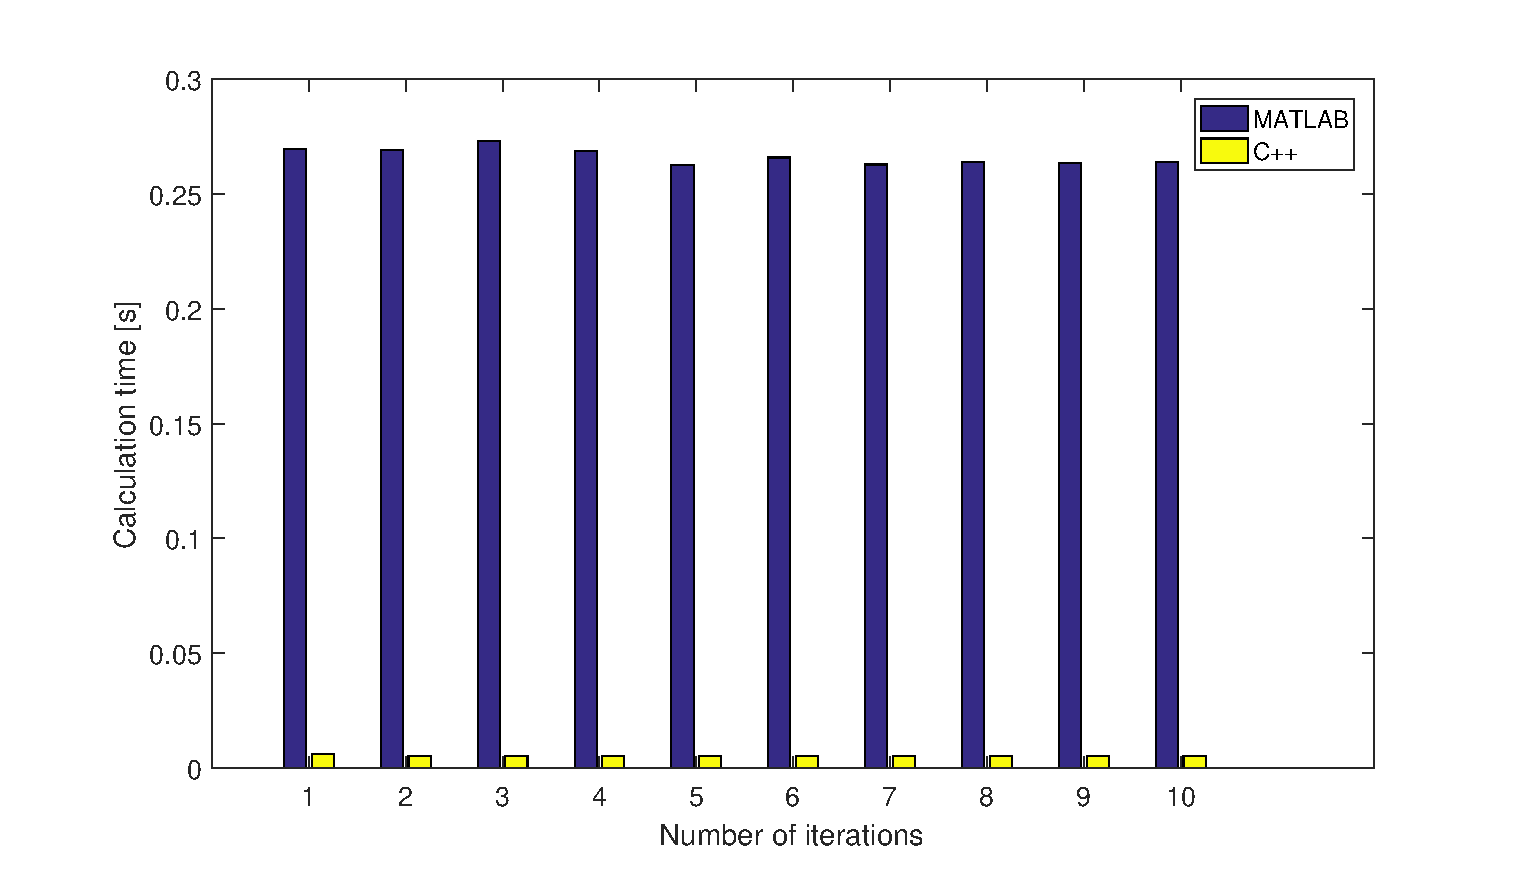
\includegraphics[width = 0.9\textwidth]{fig/MvsC_10.eps}
    \end{figure}
\end{frame}

\begin{frame}
\frametitle{Undersökta fall: Fall 1}
\begin{itemize}
    \item \textbf{Fall 1:} effekttoppar reduceras för det enskilda hushållet, men spänningstransienter för närliggande hushåll tas hänsyn till. Endast en elbil (styrbar eller icke-styrbar). Solpaneler kan finnas på hushållet med elbil.
\end{itemize}
\end{frame}

\begin{frame}
\frametitle{Undersökta fall: Fall 1}
\begin{equation*}
    \begin{aligned}
        & \underset{x}{\text{min}}
        & & \alpha \sum (P_\text{net} + x)^2 + \beta \sum \sum (U_\text{mean}-U_\text{house})^2 \\
        & \text{s.t.}
        & & 0.1 \leq \text{SoC}(t) \leq 0.9 \\
        & & - & \frac{P_\text{max}}{Q_b}\eta_b \leq \text{SoC}(t+1)-\text{SoC}(t) \leq \frac{P_\text{max}}{Q_b}\eta_b \\
        & & & 0.9 \: \text{p.u.} \leq V(t) \leq 1.1 \: \text{p.u.} \\
        & & & I(t) \leq 16 \: \text{A} \\
        & & & 0.95 \, V(t) \leq V(t+1) \leq 1.1 V(t) \\
        & & - & P_\text{max} \leq x(t) \leq P_\text{max}
    \end{aligned}
\end{equation*}
\end{frame}

% optiData1 combiplot
\begin{frame}[plain]
\Wider[10em]{
    \begin{figure}
        \centering
        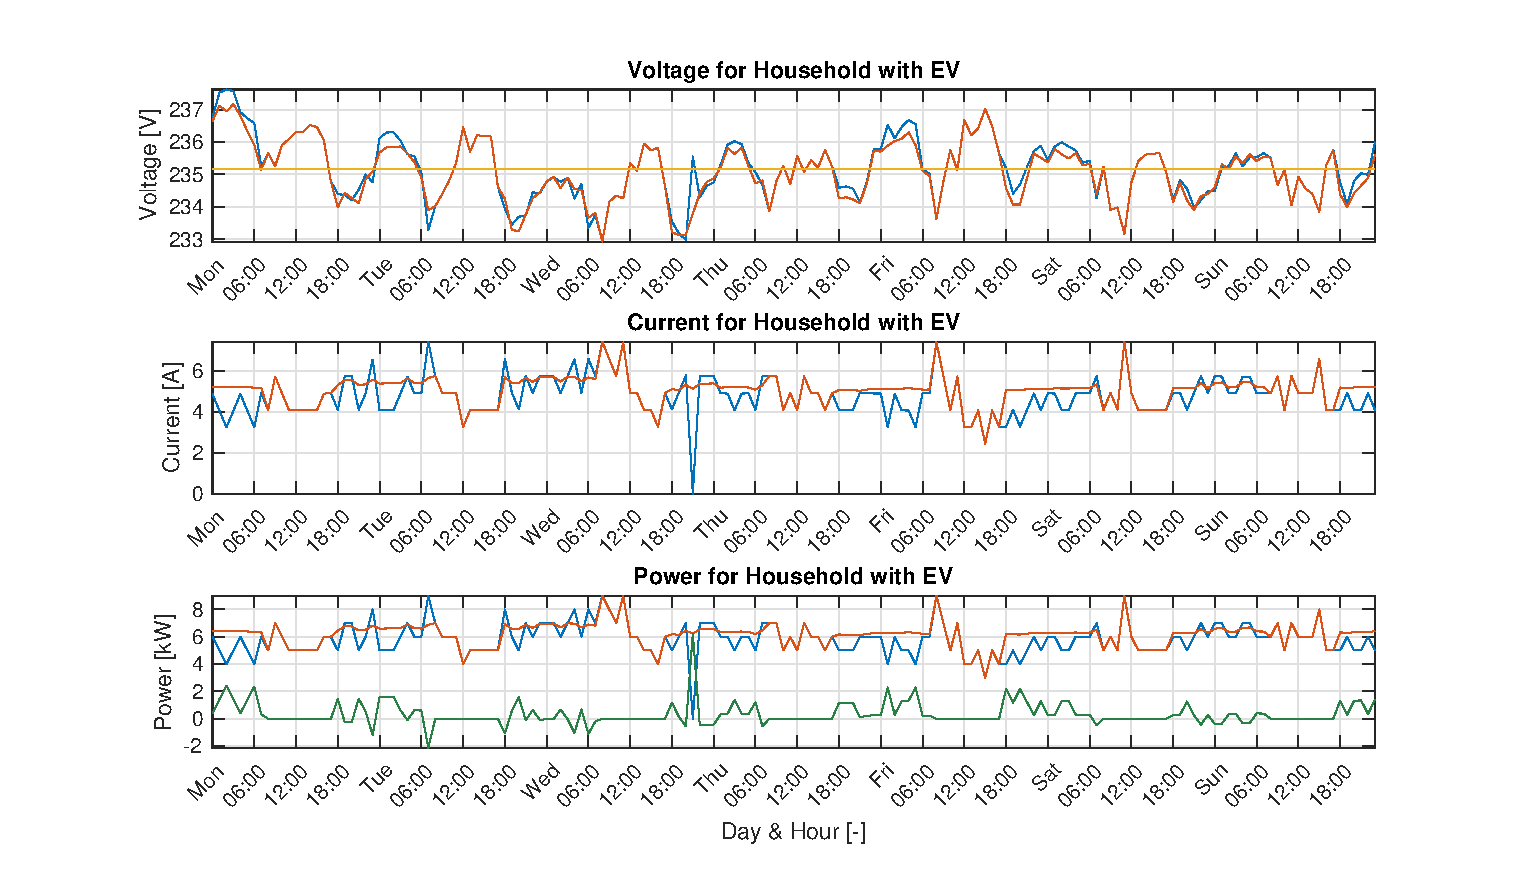
\includegraphics[scale = 0.5]{fig/combiplot1.eps} \\~\\
        Fall 1: \textcolor{myblue}{ej optimerad}, \textcolor{myred}{optimerad}, \textcolor{myyellow}{medelvärde}, \textcolor{mygreen}{batterieffekt}
    \end{figure}
    }
\end{frame}



% optiData1 SoC plot
\begin{frame}[plain]
\Wider[10em]{
    \begin{figure}
        \centering
        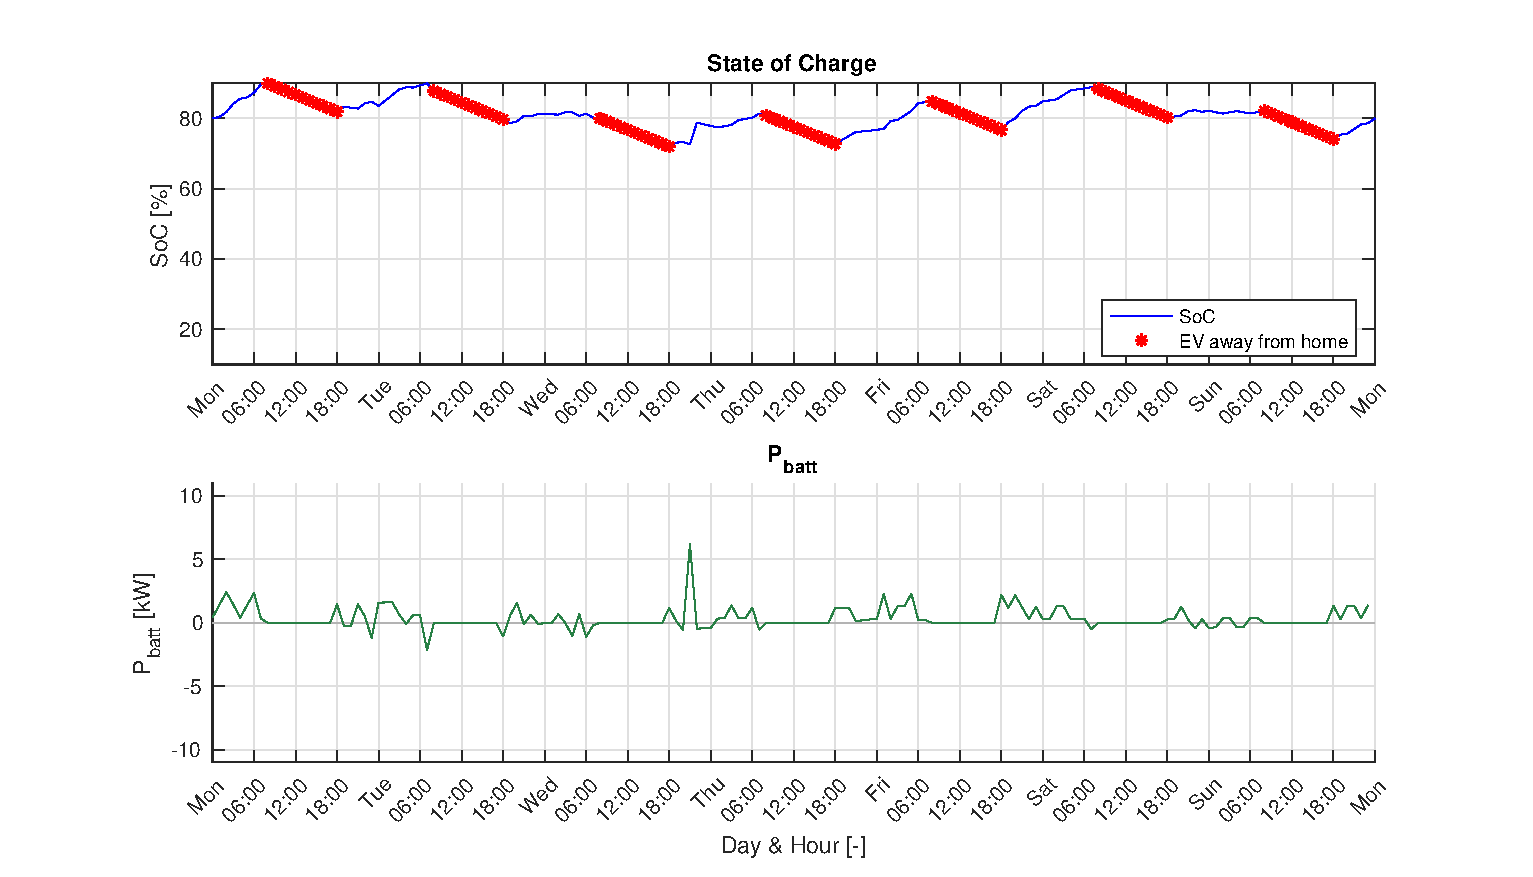
\includegraphics[width=0.83\linewidth]{fig/soc1.eps} \\~\\
        Fall 1
    \end{figure}
    }
\end{frame}

% optiData1 voltage plot
\begin{frame}[plain]
\Wider[10em]{
    \begin{figure}
        \centering
        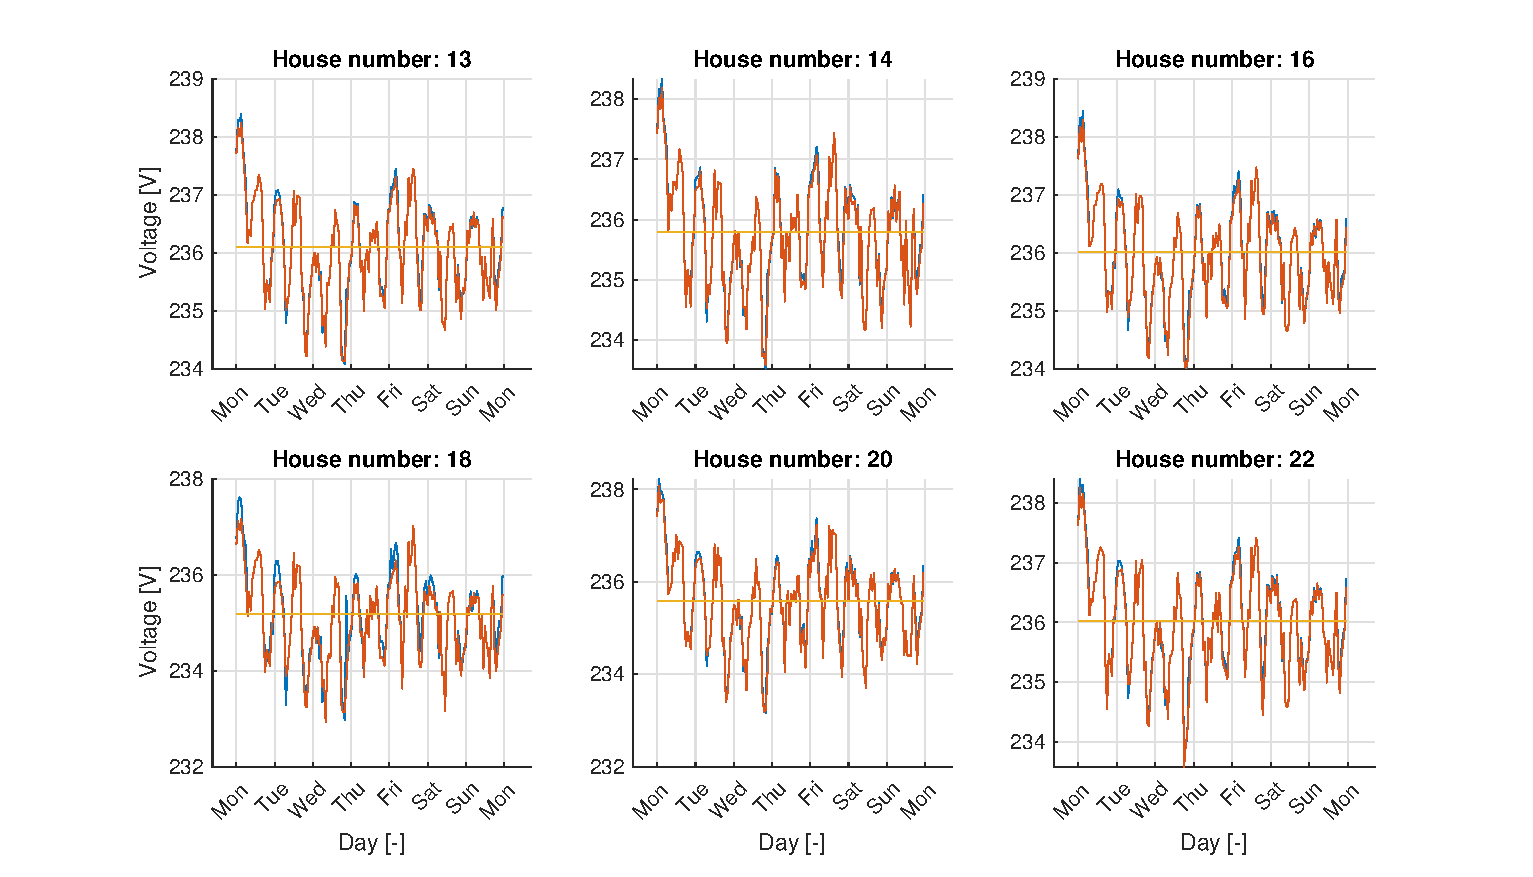
\includegraphics[scale = 0.5]{fig/volt1.eps} \\~\\
        Fall 1: \textcolor{myblue}{ej optimerad}, \textcolor{myred}{optimerad}, \textcolor{myyellow}{medelvärde}
    \end{figure}
    }
\end{frame}

% optiData2 combiplot
\begin{frame}[plain]
\Wider[10em]{
    \begin{figure}
        \centering
        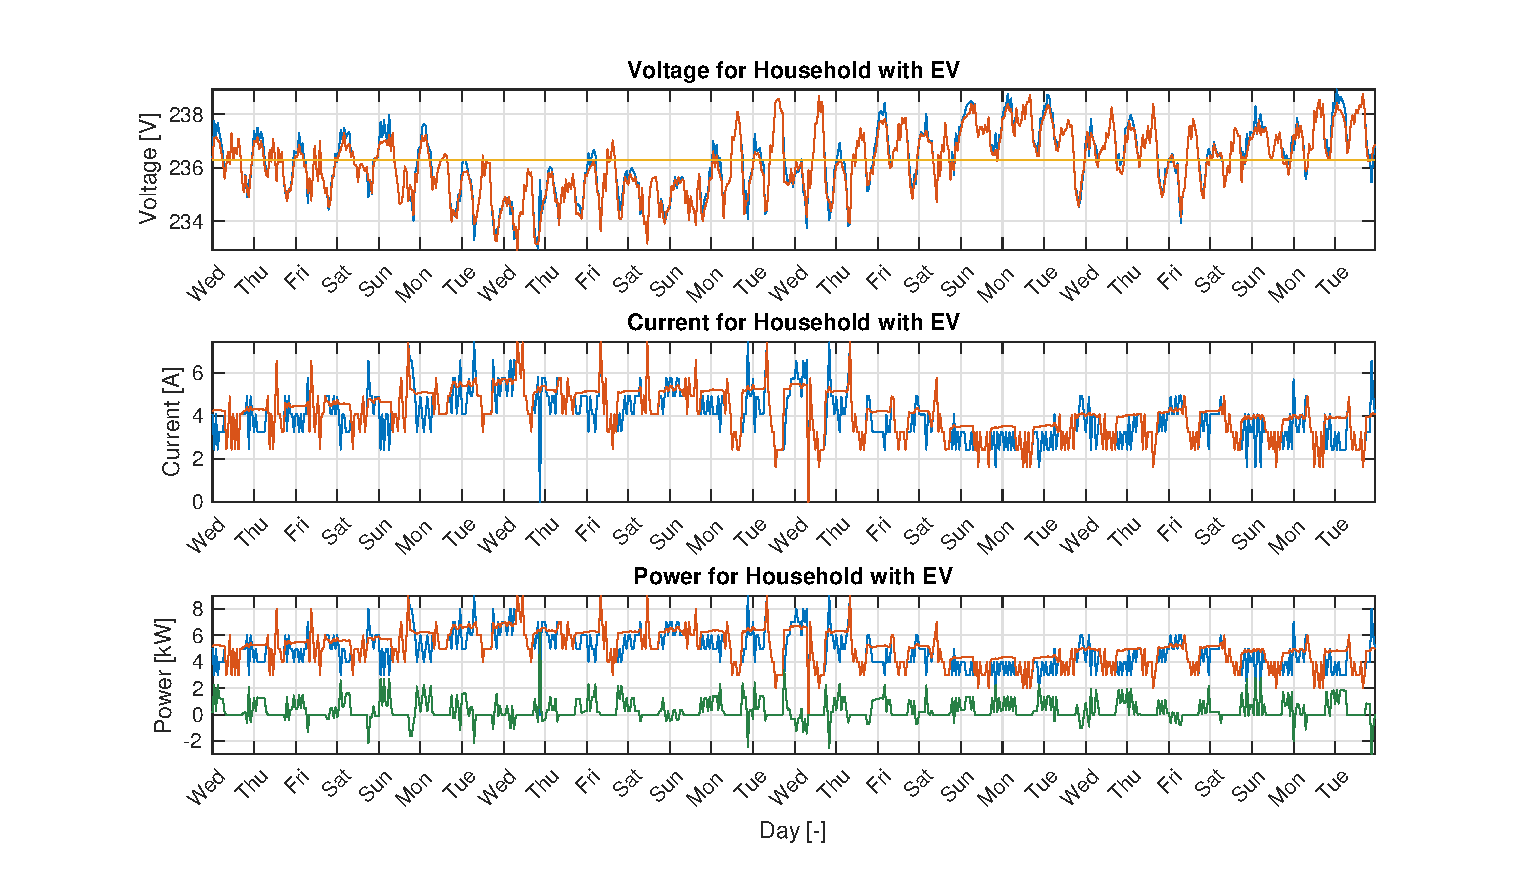
\includegraphics[scale = 0.5]{fig/combiplot2.eps} \\~\\
        Fall 1: \textcolor{myblue}{ej optimerad}, \textcolor{myred}{optimerad}, \textcolor{myyellow}{medelvärde}, \textcolor{mygreen}{batterieffekt}
    \end{figure}
    }
\end{frame}

% optiData2 SoC plot
\begin{frame}[plain]
\Wider[10em]{
    \begin{figure}
        \centering
        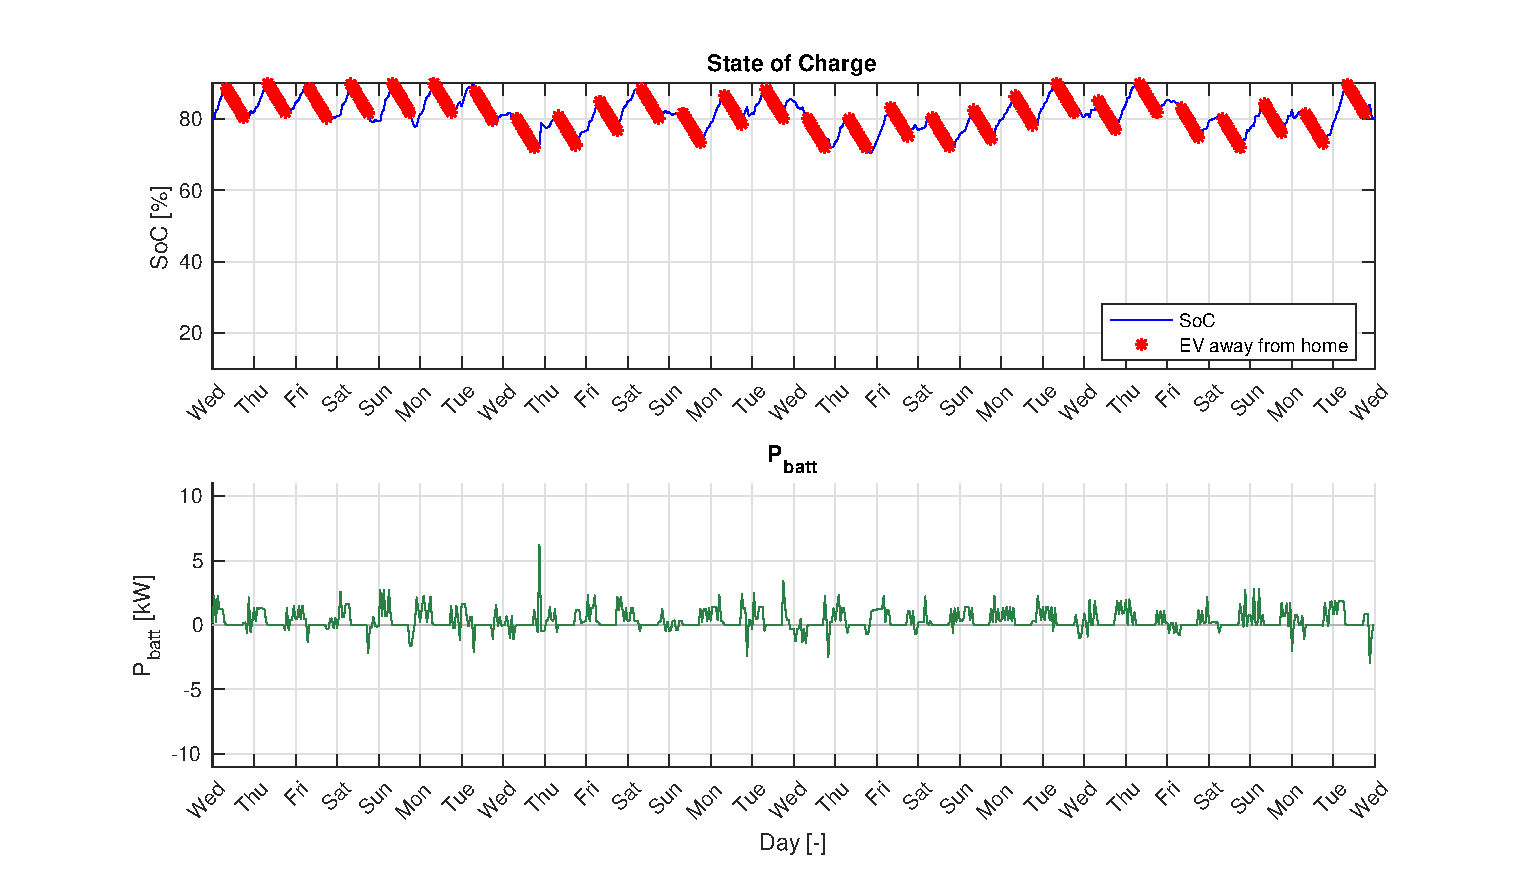
\includegraphics[width=0.83\linewidth]{fig/soc2.eps} \\~\\
        Fall 1
    \end{figure}
    }
\end{frame}

\begin{frame}
\frametitle{Undersökta fall: Fall 2}
    \begin{itemize}
        \item \textbf{Fall 2:} enbart spänningstransienter tas hänsyn till. Undersöker möjligheter till att stabilisera elnätet med styrbara elbilar. Flera elbilar kan finnas (styrbara och icke-styrbara). Solpaneler kan vara placerade på ett antal hushåll.
    \end{itemize}
\end{frame}

\begin{frame}
\frametitle{Undersökta fall: Fall 2}
\begin{equation*}
    \begin{aligned}
        & \underset{x}{\text{min}}
        & & \beta \sum \sum (U_\text{mean}-U_\text{house})^2 \\
        & \text{s.t.}
        & & 0.1 \leq \text{SoC}(t) \leq 0.9 \\
        & & - & \frac{P_\text{max}}{Q_b}\eta_b \leq \text{SoC}(t+1)-\text{SoC}(t) \leq \frac{P_\text{max}}{Q_b}\eta_b \\
        & & & 0.9 \: \text{p.u.} \leq V(t) \leq 1.1 \: \text{p.u.} \\
        & & & I(t) \leq 16 \: \text{A} \\
        & & & 0.95 \, V(t) \leq V(t+1) \leq 1.1 V(t) \\
        & & - & P_\text{max} \leq x(t) \leq P_\text{max}
    \end{aligned}
\end{equation*}
\end{frame}

\begin{frame}
\frametitle{Undersökta fall: Fall 2}
Styrbar elbil vid hushåll 18. Spänningsvariationer ska minimeras vid varje hushåll.
    \begin{figure}
        \centering
        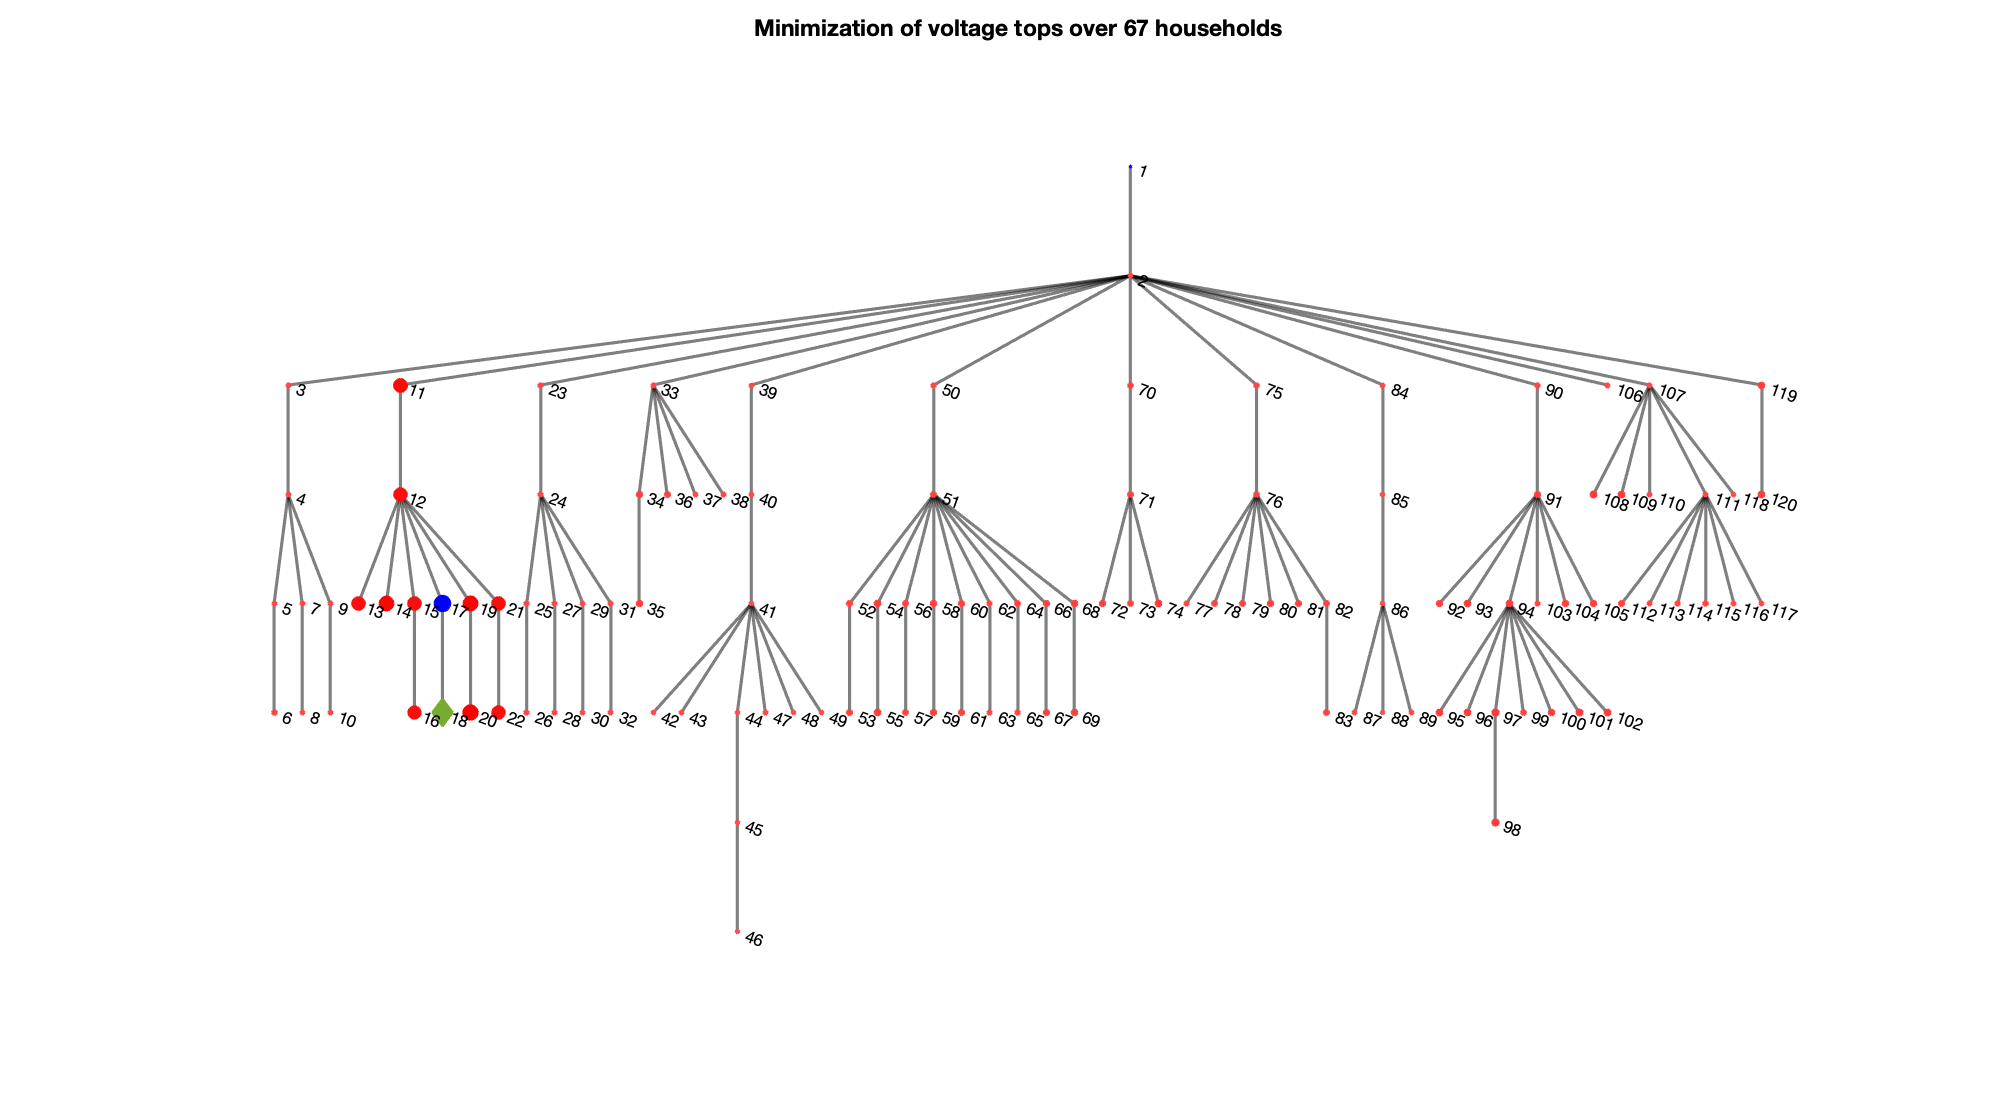
\includegraphics[width = 0.83\linewidth]{templates/fig/tree_Uall_18_pdf.pdf}
    \end{figure}
\end{frame}

% Treeplot color for case 2
\begin{frame}
\frametitle{Undersökta fall: Fall 2}
Styrbar elbil vid hushåll 18. Spänningsvariationer ska minimeras vid hushåll under samma gren.
    \begin{figure}
        \centering
        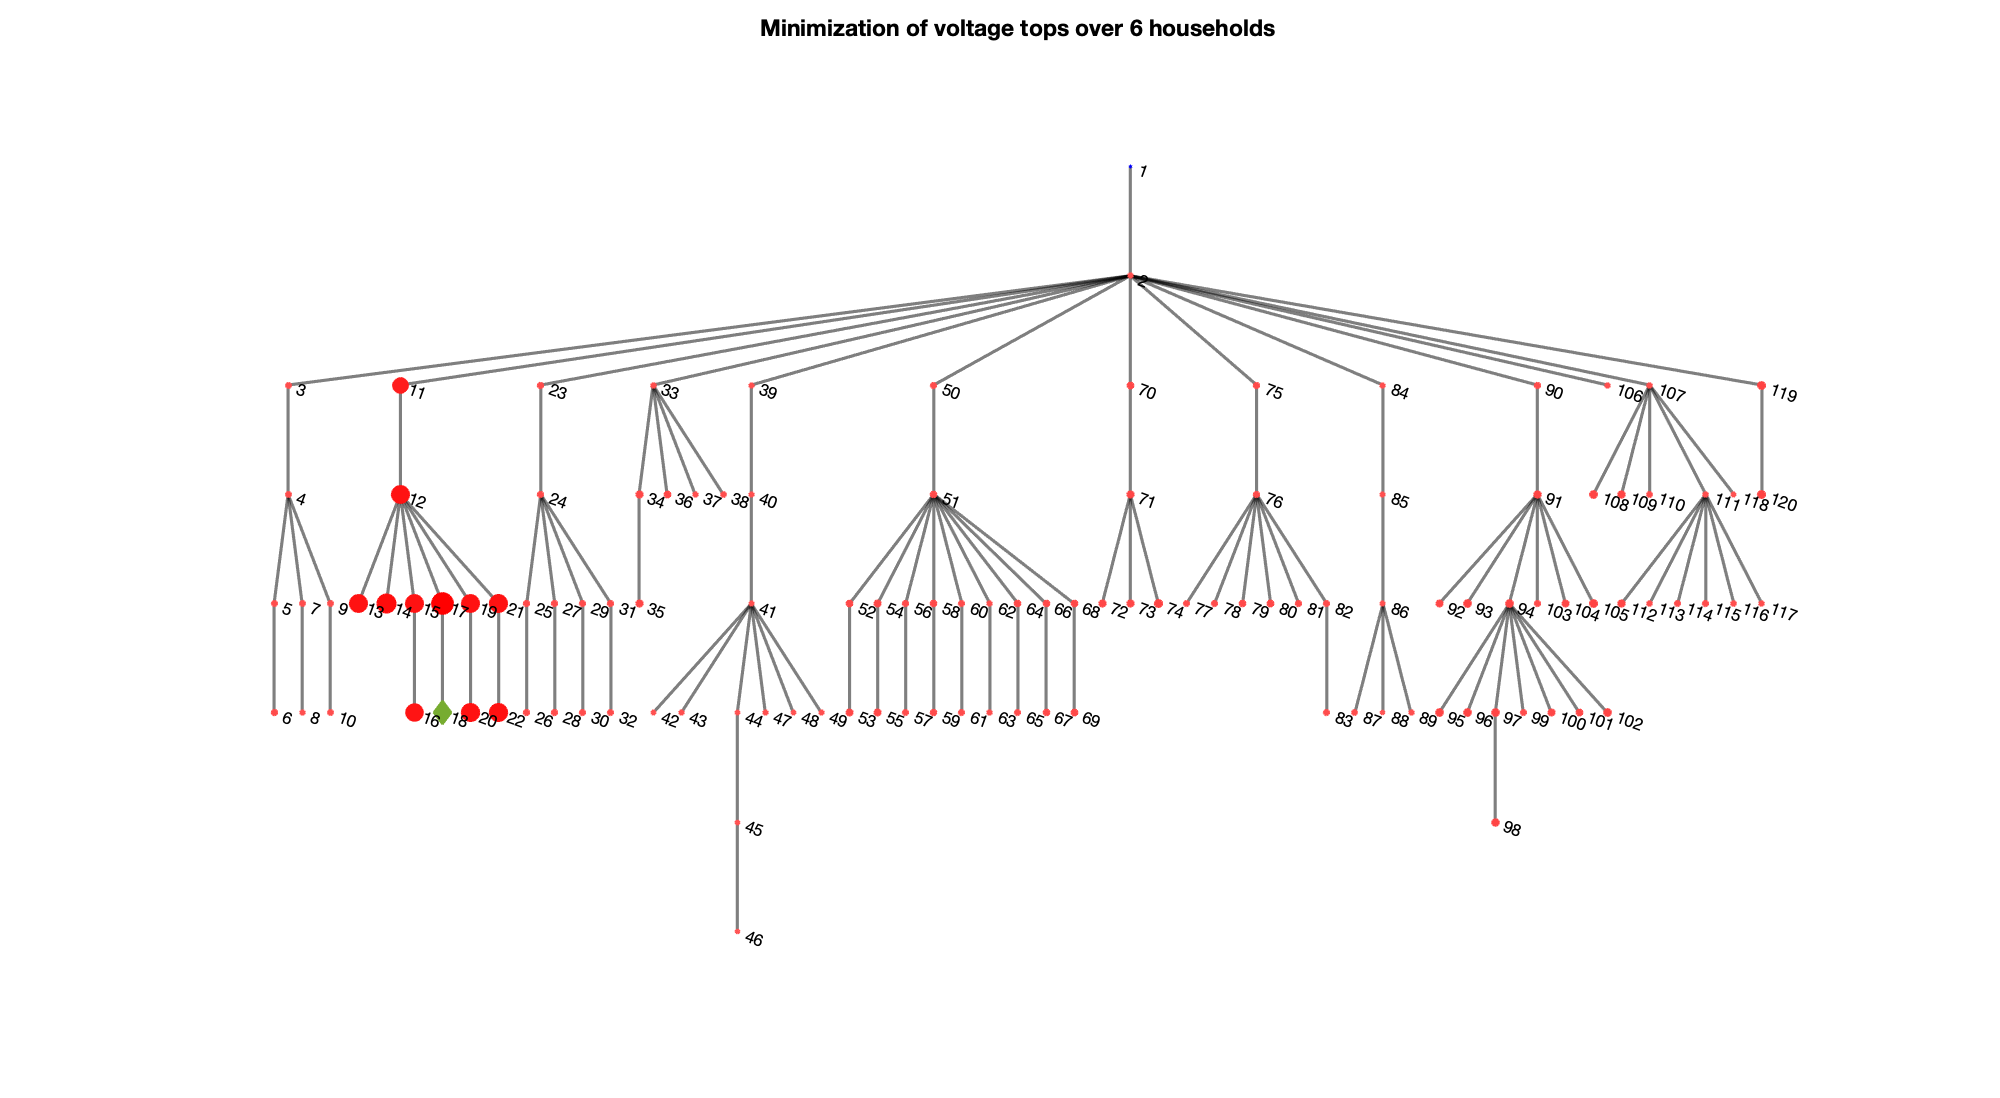
\includegraphics[width = 0.83\linewidth]{templates/fig/tree_Uclust_18_pdf.pdf}
    \end{figure}
\end{frame}

\begin{frame}
\frametitle{Undersökta fall: Fall 2}
Styrbar elbil vid hushåll 73. Spänningsvariationer ska minimeras vid varje hushåll.
    \begin{figure}
        \centering
        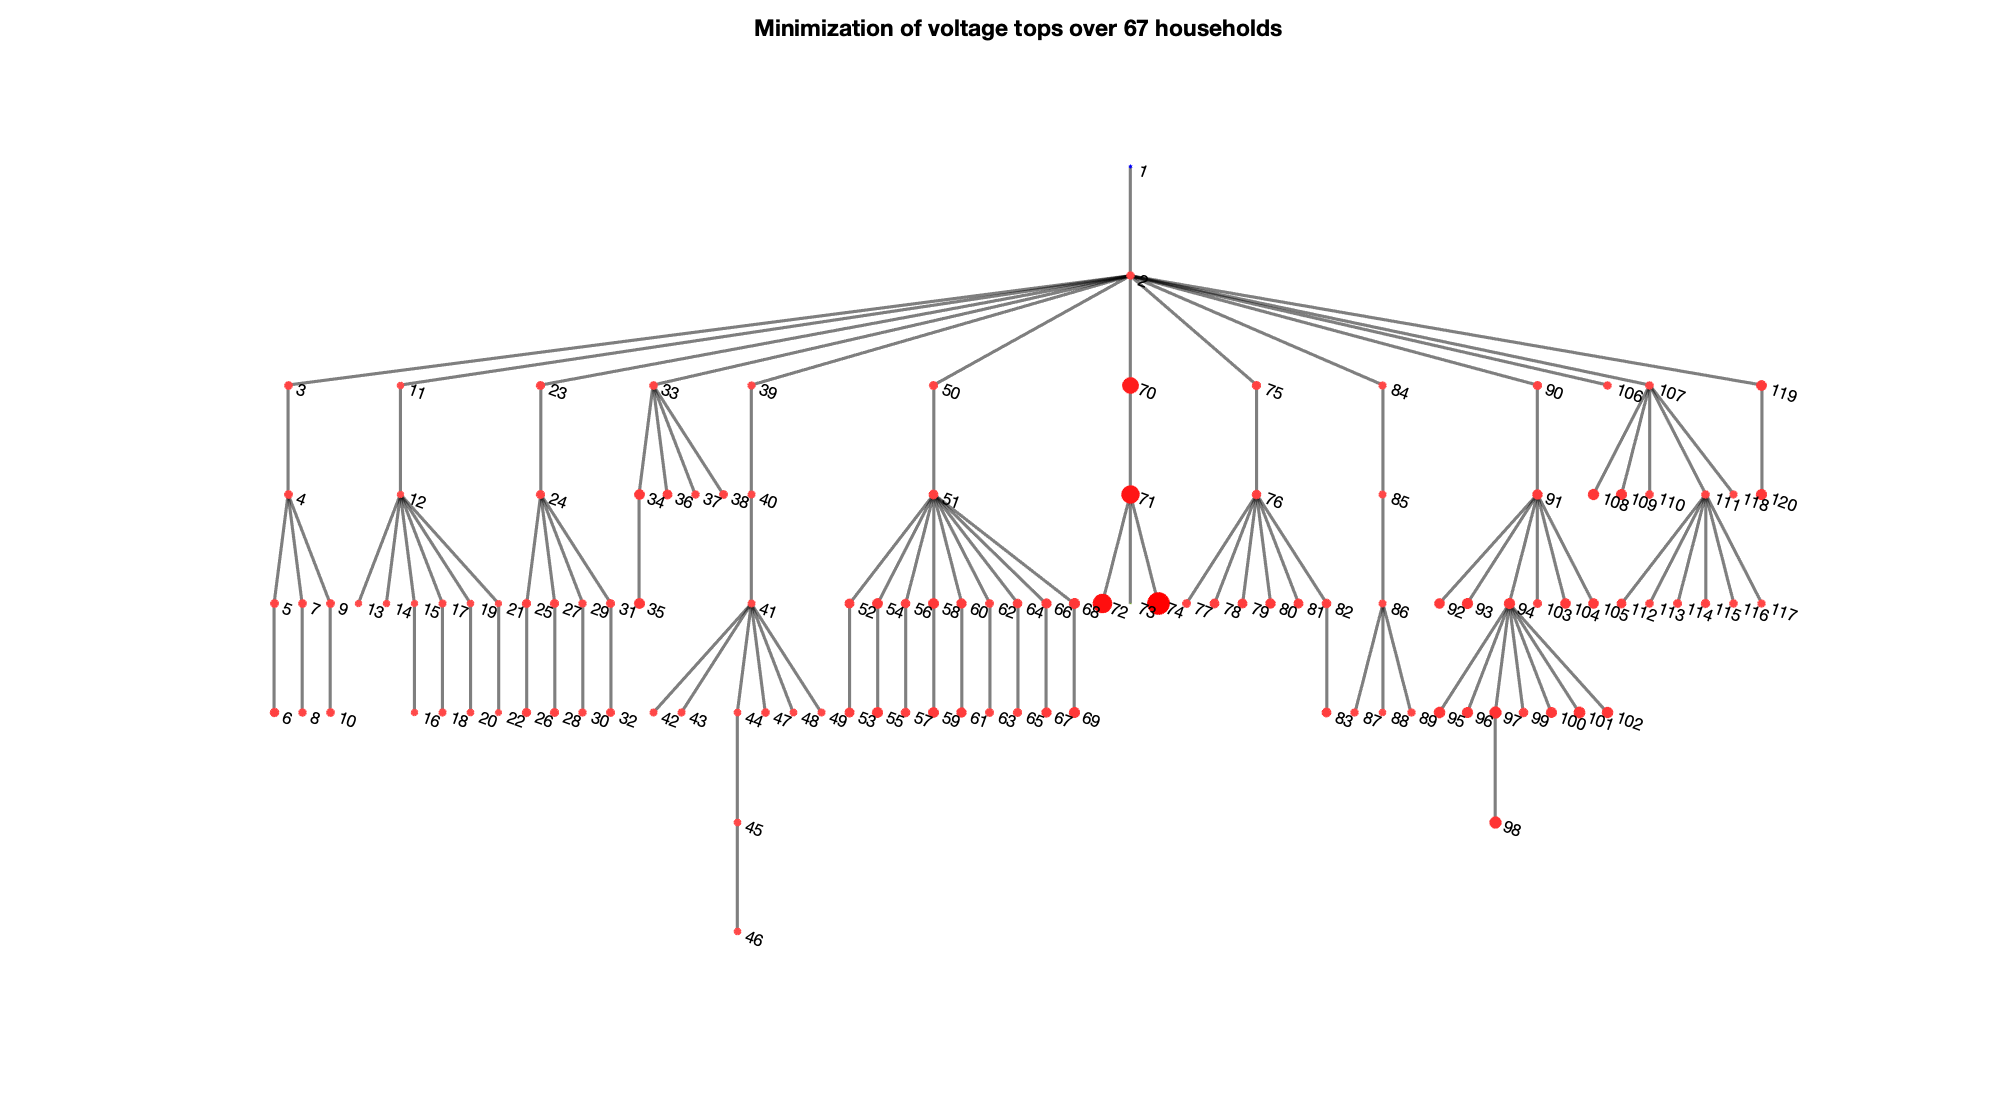
\includegraphics[width = 0.83\linewidth]{templates/fig/tree_Uall_73_pdf.pdf}
    \end{figure}
\end{frame}

\begin{frame}
\frametitle{Undersökta fall: Fall 2}
Styrbar elbil vid hushåll 73. Spänningsvariationer ska minimeras vid hushåll under samma gren.
    \begin{figure}
        \centering
        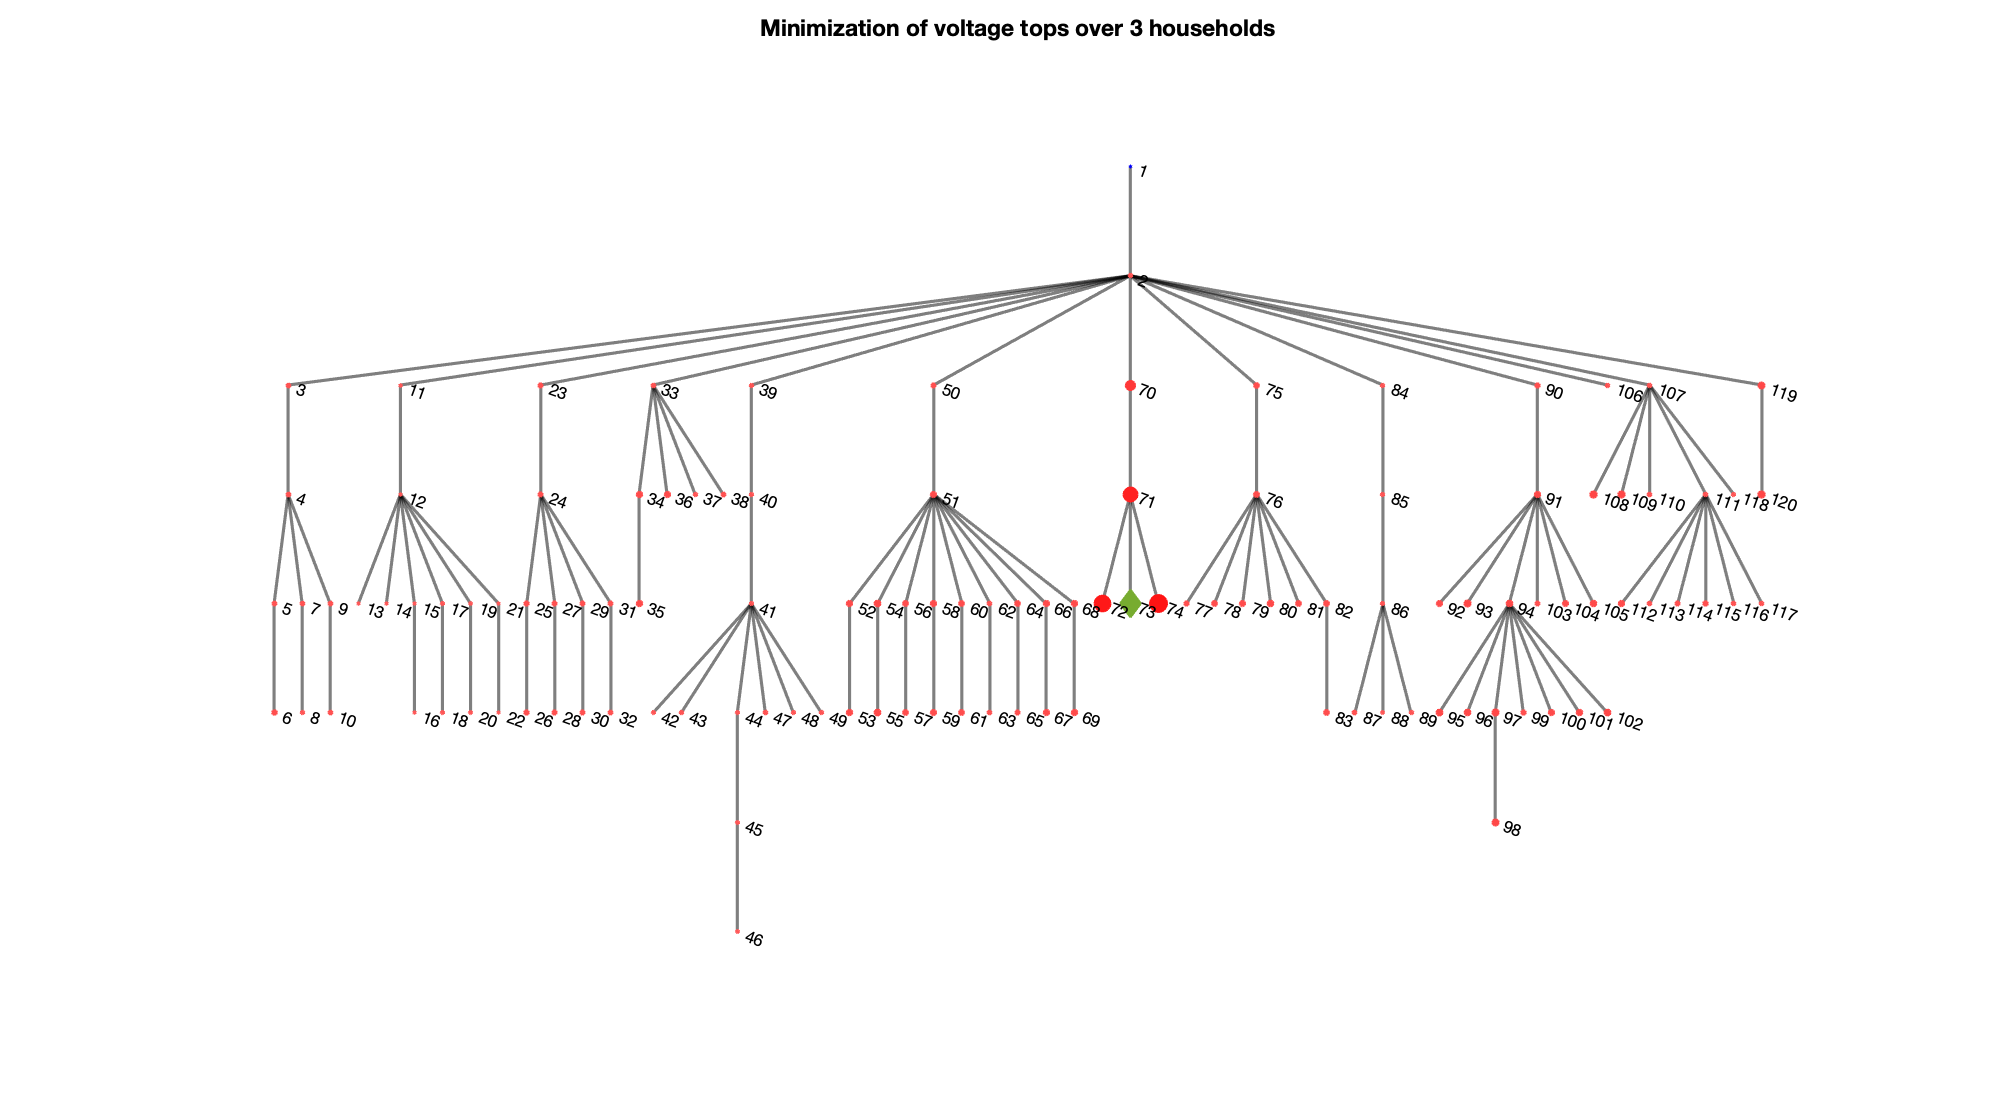
\includegraphics[width = 0.83\linewidth]{templates/fig/tree_Uclust_73_pdf.pdf}
    \end{figure}
\end{frame}

% optiData3 combiplot
\begin{frame}[plain]
\Wider[10em]{
    \begin{figure}
        \centering
        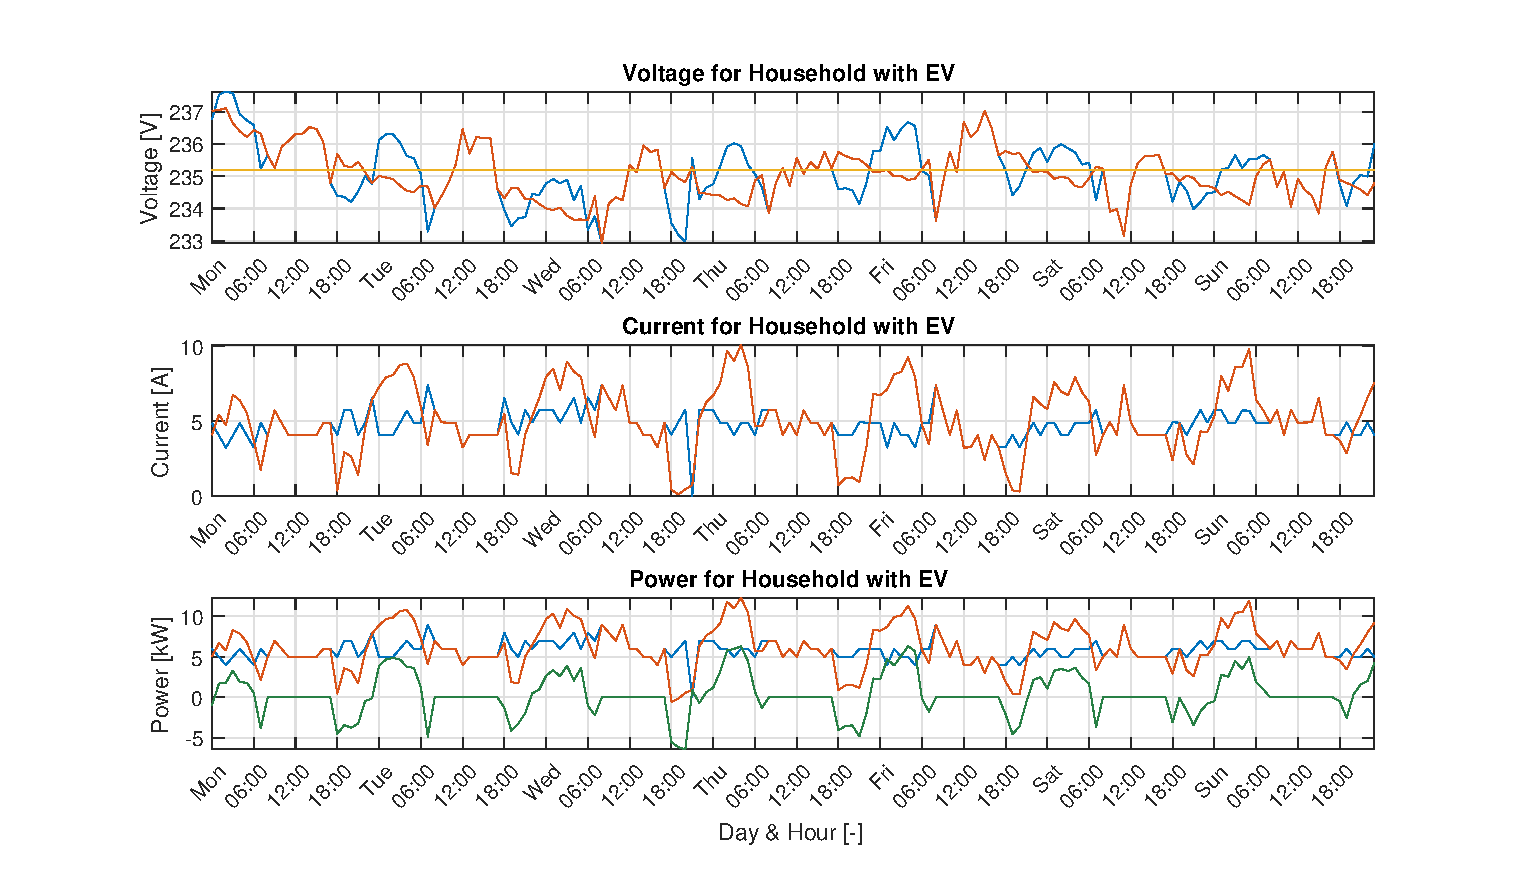
\includegraphics[scale = 0.5]{fig/combiplot3.eps} \\~\\
        Fall 2: \textcolor{myblue}{ej optimerad}, \textcolor{myred}{optimerad}, \textcolor{myyellow}{medelvärde}, \textcolor{mygreen}{batterieffekt}
    \end{figure}
    }
\end{frame}

% optiData3 SoC plot
\begin{frame}[plain]
\Wider[10em]{
    \begin{figure}
        \centering
        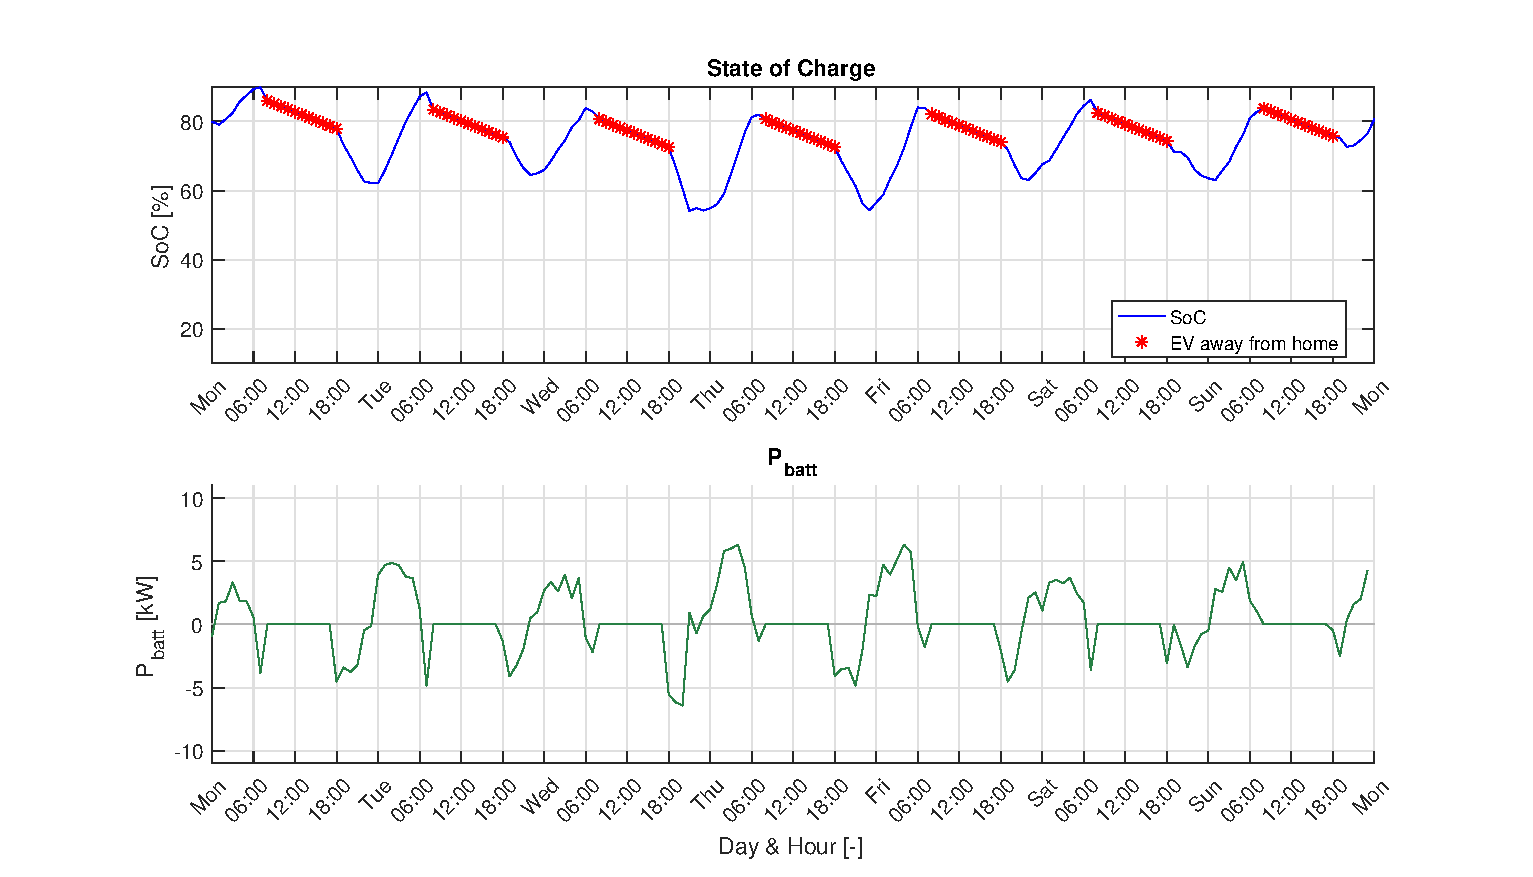
\includegraphics[width=0.83\linewidth]{fig/soc3.eps} \\~\\
        Fall 2
    \end{figure}
    }
\end{frame}

% optiData3 voltage plot
\begin{frame}[plain]
\Wider[10em]{
    \begin{figure}
        \centering
        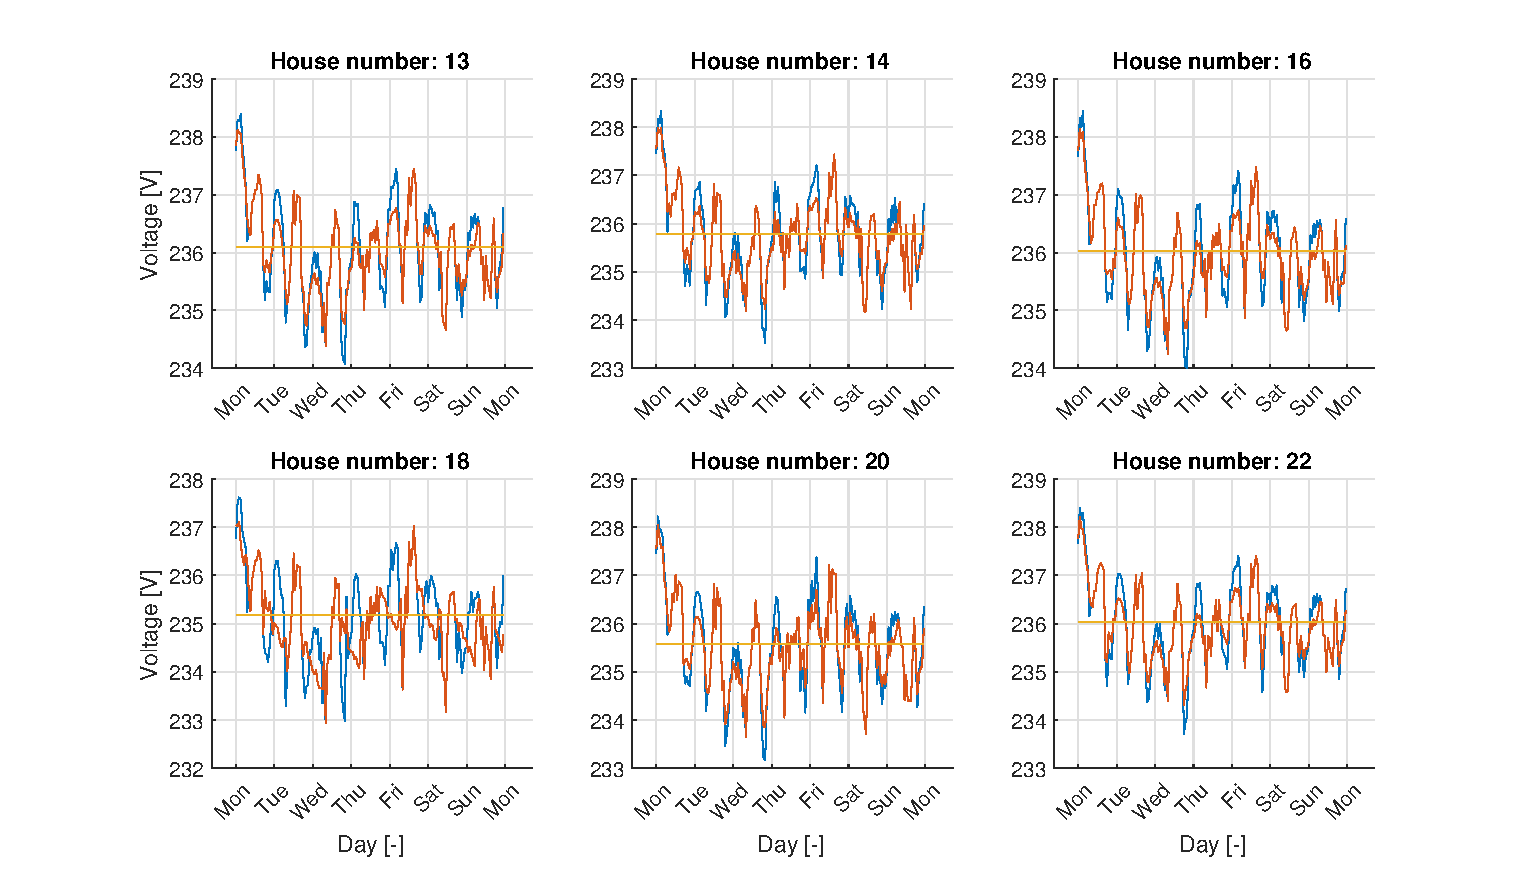
\includegraphics[scale = 0.5]{fig/volt3.eps} \\~\\
        Fall 2: \textcolor{myblue}{ej optimerad}, \textcolor{myred}{optimerad}, \textcolor{myyellow}{medelvärde}
    \end{figure}
    }
\end{frame}


% optiData4 combiplot
\begin{frame}[plain]
\Wider[10em]{
    \begin{figure}
        \centering
        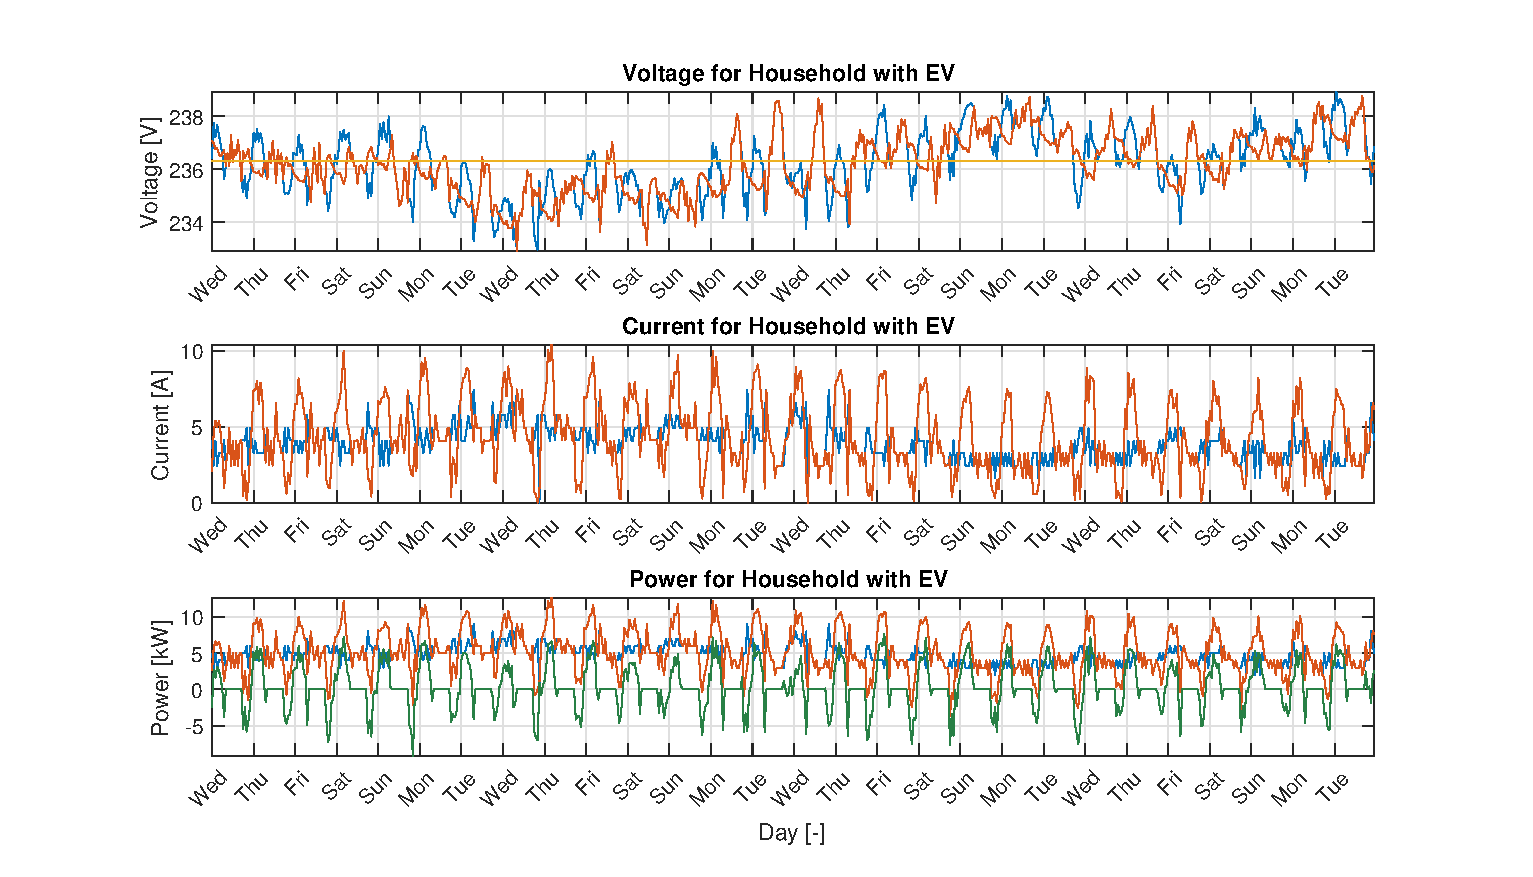
\includegraphics[scale = 0.5]{fig/combiplot4.eps} \\~\\
        Fall 2: \textcolor{myblue}{ej optimerad}, \textcolor{myred}{optimerad}, \textcolor{myyellow}{medelvärde}, \textcolor{mygreen}{batterieffekt}
    \end{figure}
    }
\end{frame}

% optiData4 SoC plot
\begin{frame}[plain]
\Wider[10em]{
    \begin{figure}
        \centering
        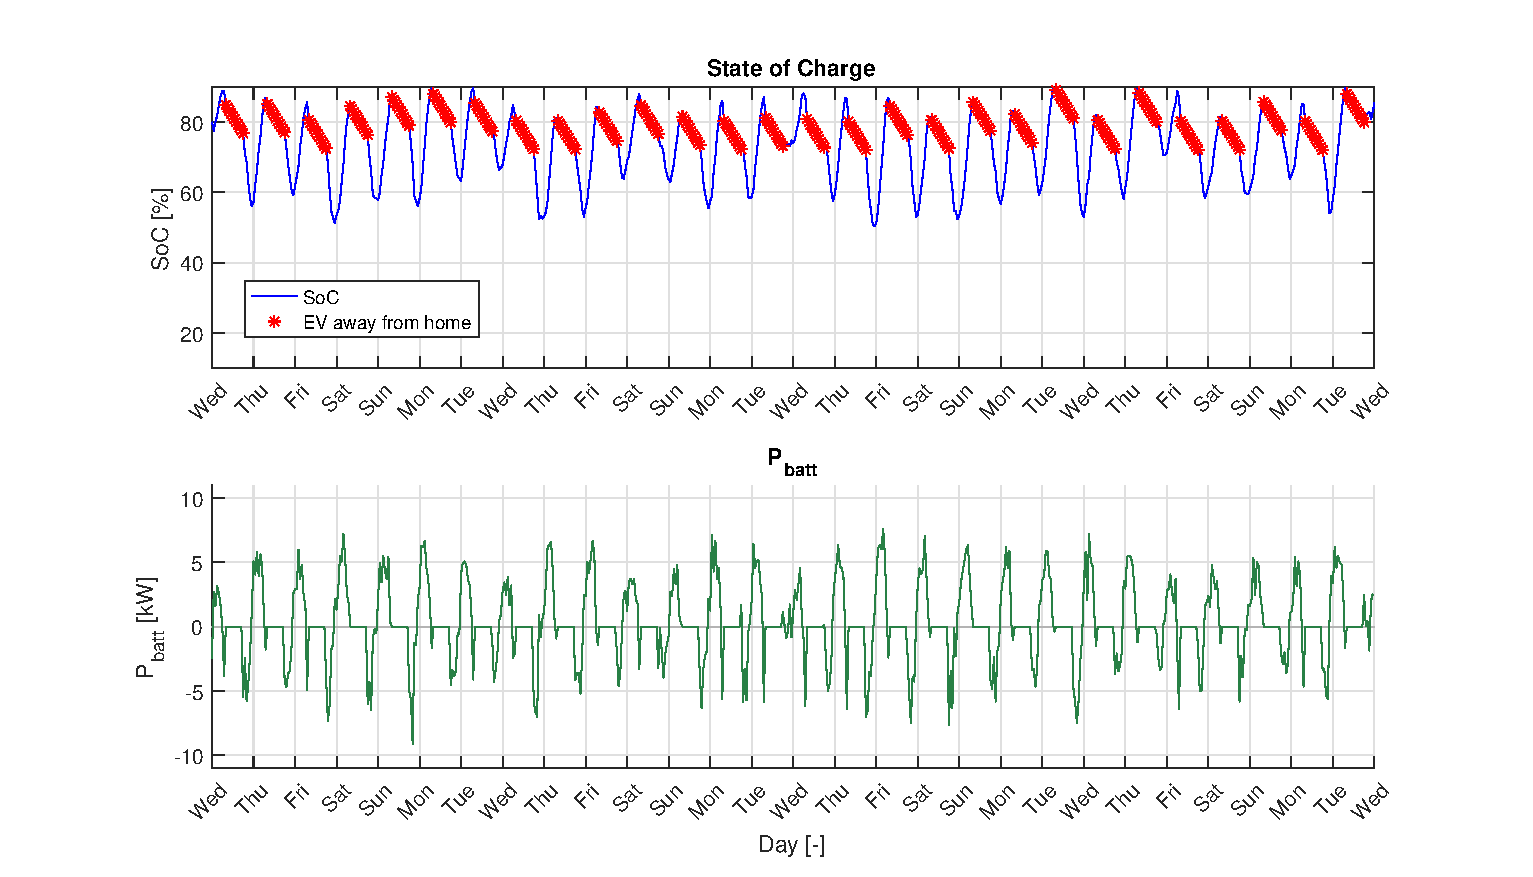
\includegraphics[scale = 0.5]{fig/soc4.eps} \\~\\
        Fall 2
    \end{figure}
    }
\end{frame}

% optiData5 combiplot
\begin{frame}[plain]
\Wider[10em]{
    \begin{figure}
        \centering
        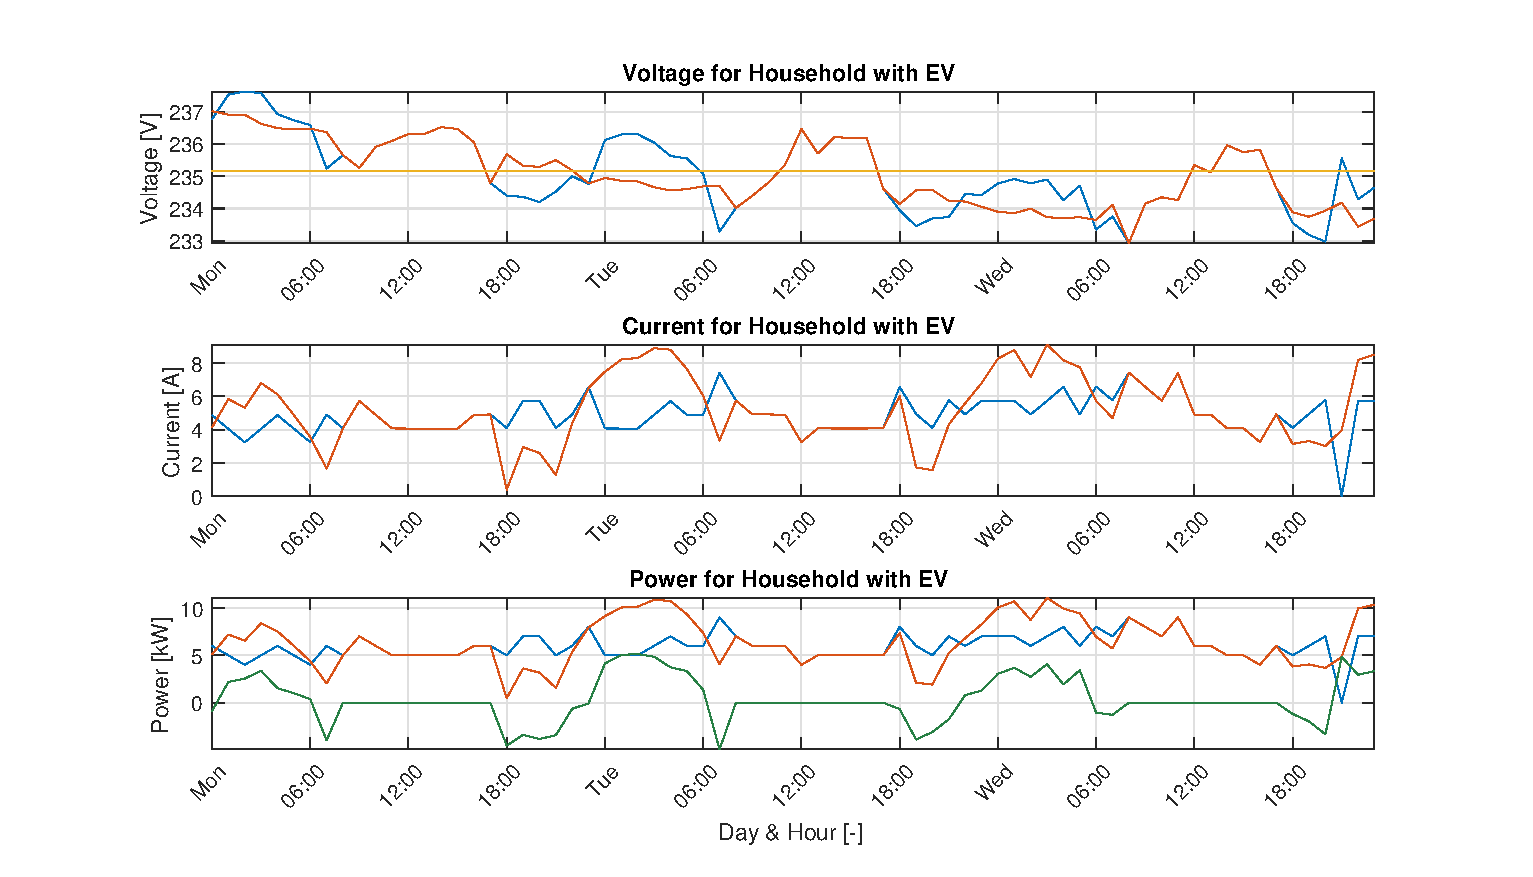
\includegraphics[scale = 0.5]{fig/combiplot5.eps} \\~\\
        Fall 2, utan PV: \textcolor{myblue}{ej optimerad}, \textcolor{myred}{optimerad}, \textcolor{myyellow}{medelvärde}, \textcolor{mygreen}{batterieffekt}
    \end{figure}
    }
\end{frame}

% optiData5 SoC plot
\begin{frame}[plain]
\Wider[10em]{
    \begin{figure}
        \centering
        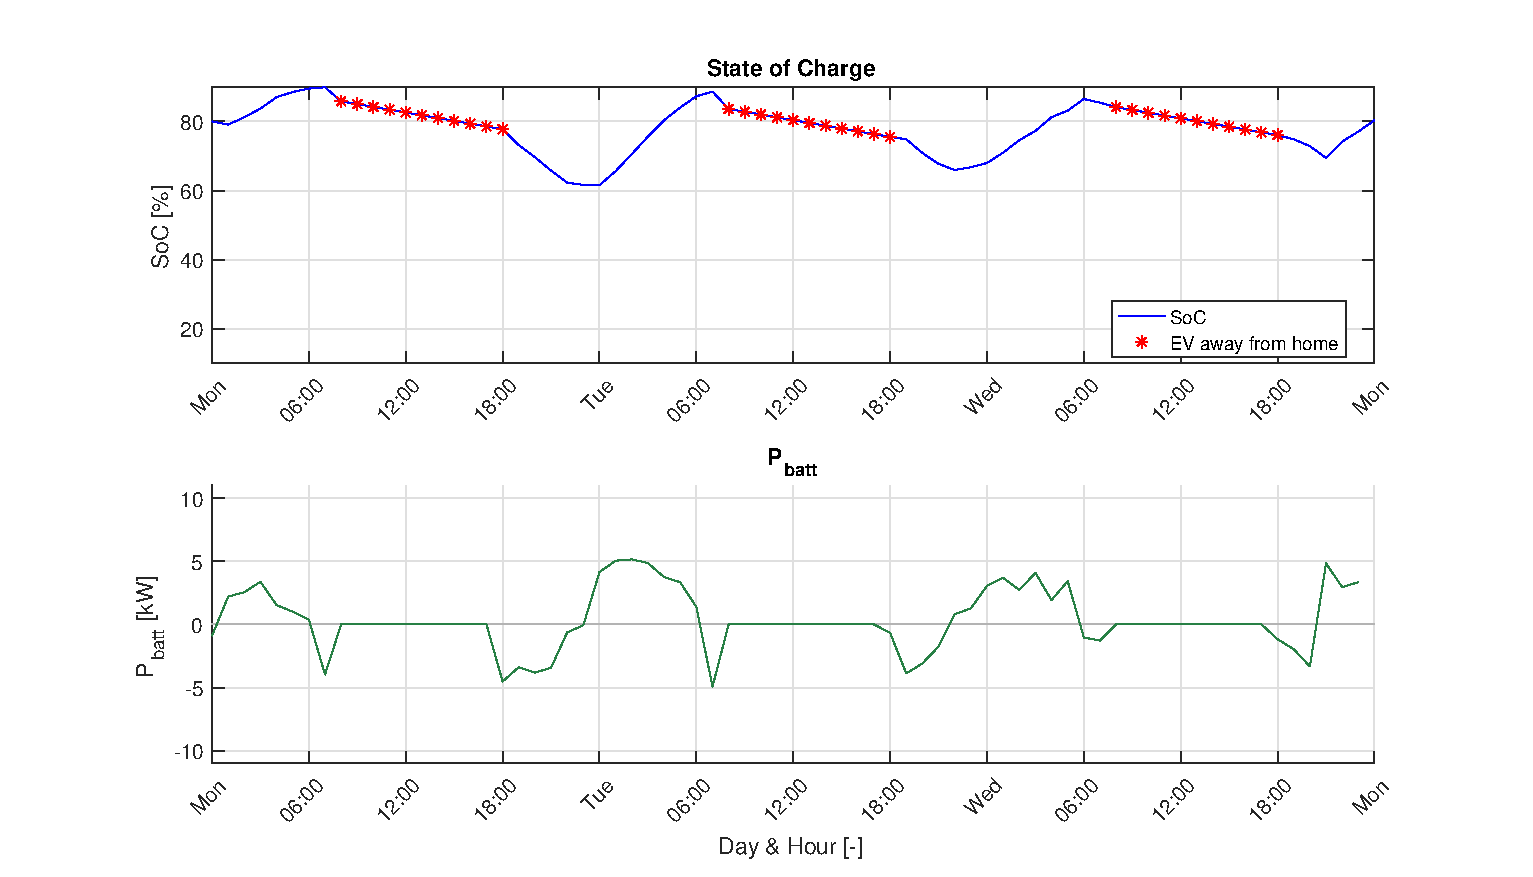
\includegraphics[scale = 0.5]{fig/soc5.eps} \\~\\
        Fall 2, utan PV
    \end{figure}
    }
\end{frame}

% optiData5 voltage plot
\begin{frame}[plain]
\Wider[10em]{
    \begin{figure}
        \centering
        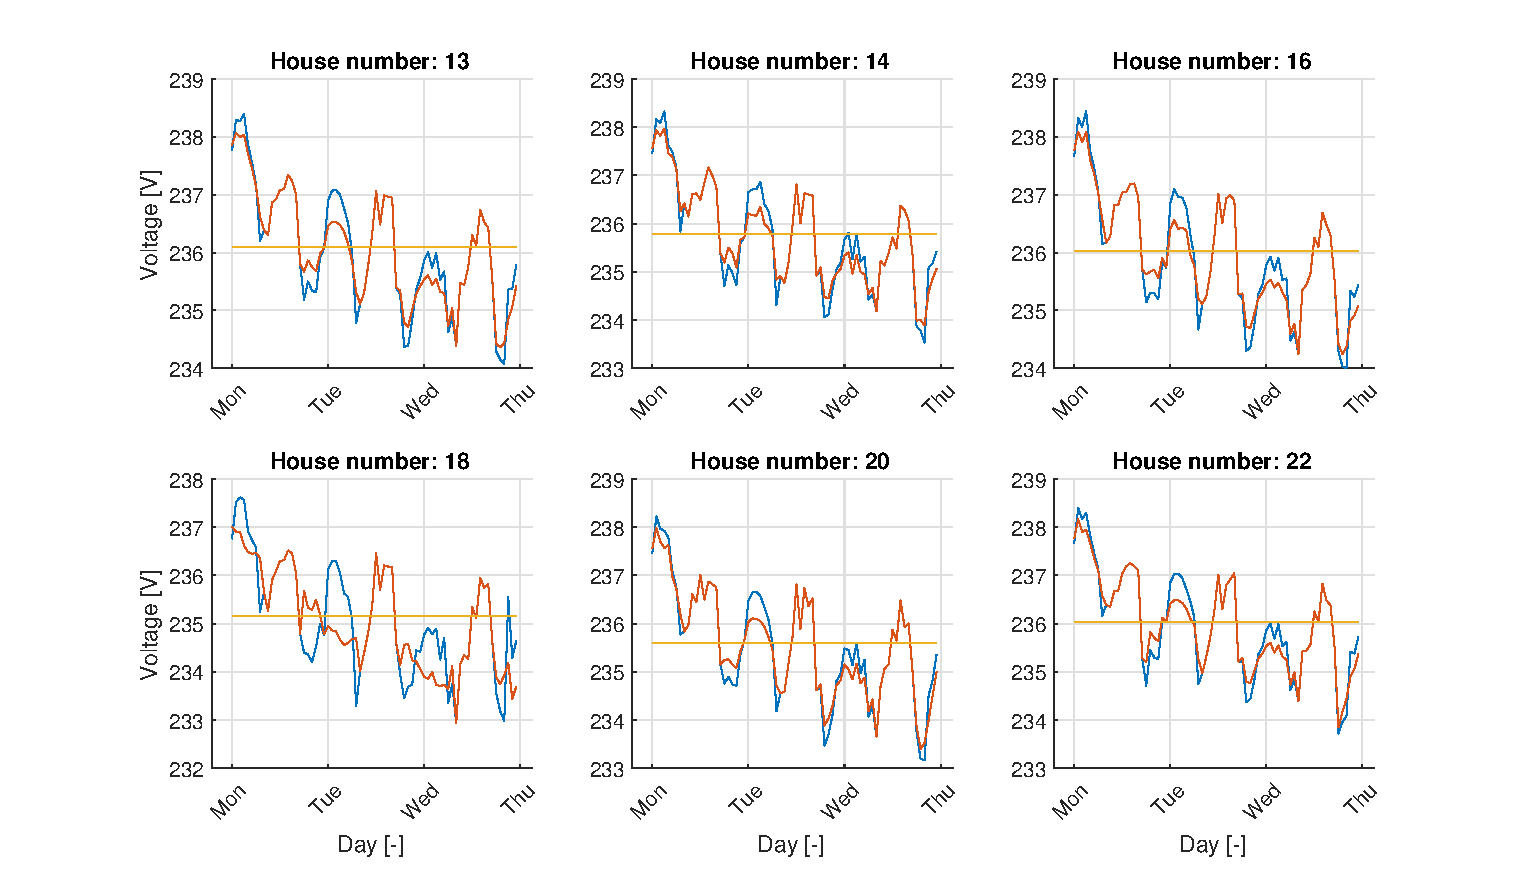
\includegraphics[scale = 0.5]{fig/volt5.eps} \\~\\
        Fall 2, utan PV: \textcolor{myblue}{ej optimerad}, \textcolor{myred}{optimerad}, \textcolor{myyellow}{medelvärde}
    \end{figure}
    }
\end{frame}

% optiData6 combiplot
\begin{frame}[plain]
\Wider[10em]{
    \begin{figure}
        \centering
        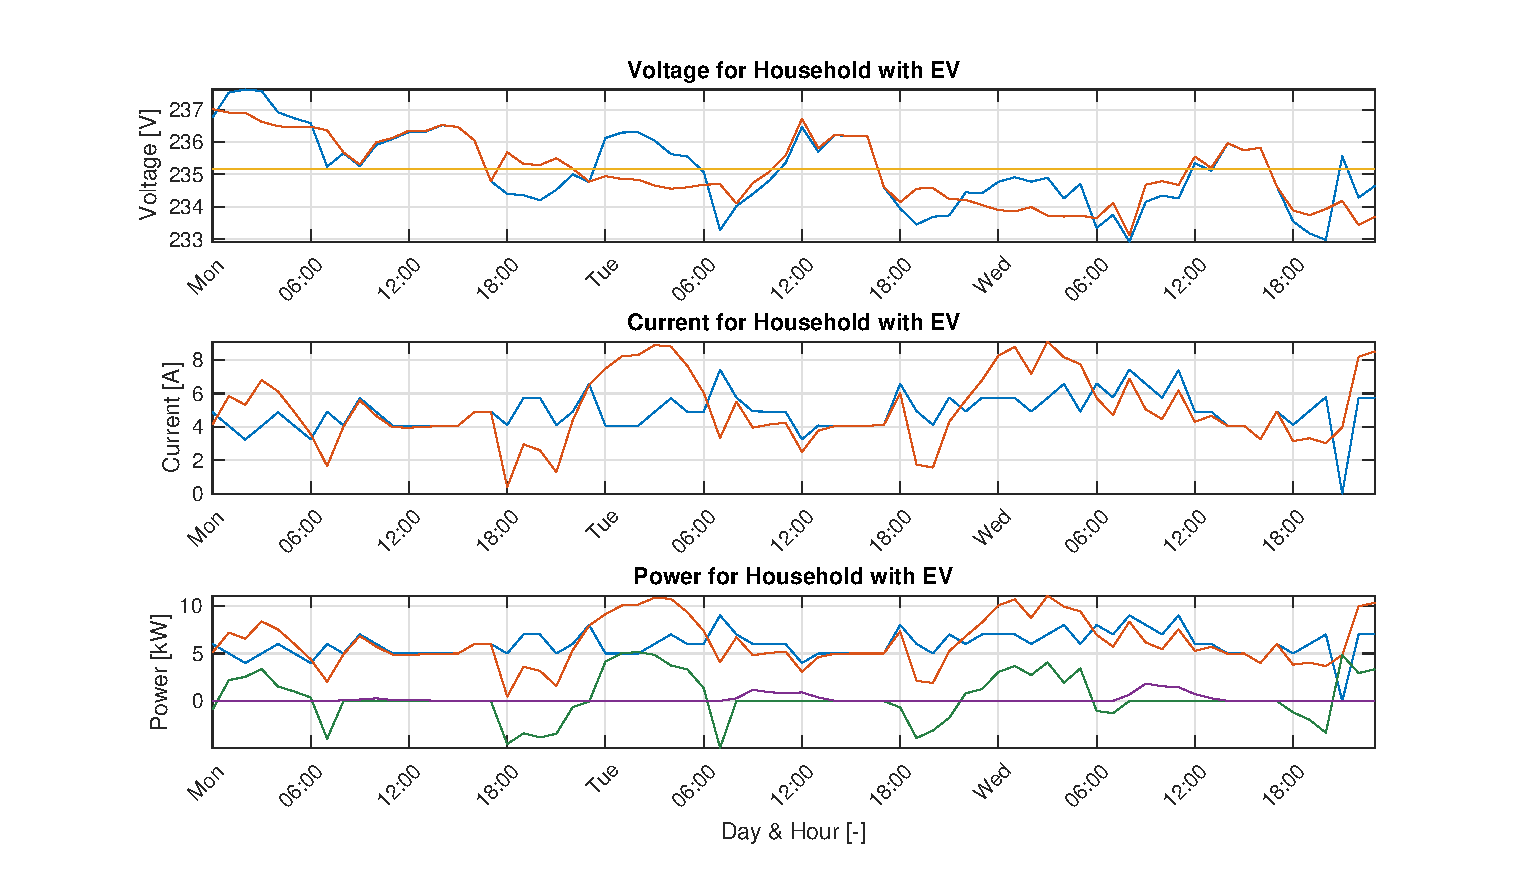
\includegraphics[scale = 0.5]{fig/combiplot6.eps} \\~\\
        Fall 2, med PV: \textcolor{myblue}{ej optimerad}, \textcolor{myred}{optimerad}, \textcolor{myyellow}{medelvärde}, \textcolor{mygreen}{batterieffekt}
    \end{figure}
    }
\end{frame}

% optiData5 SoC plot
\begin{frame}[plain]
\Wider[10em]{
    \begin{figure}
        \centering
        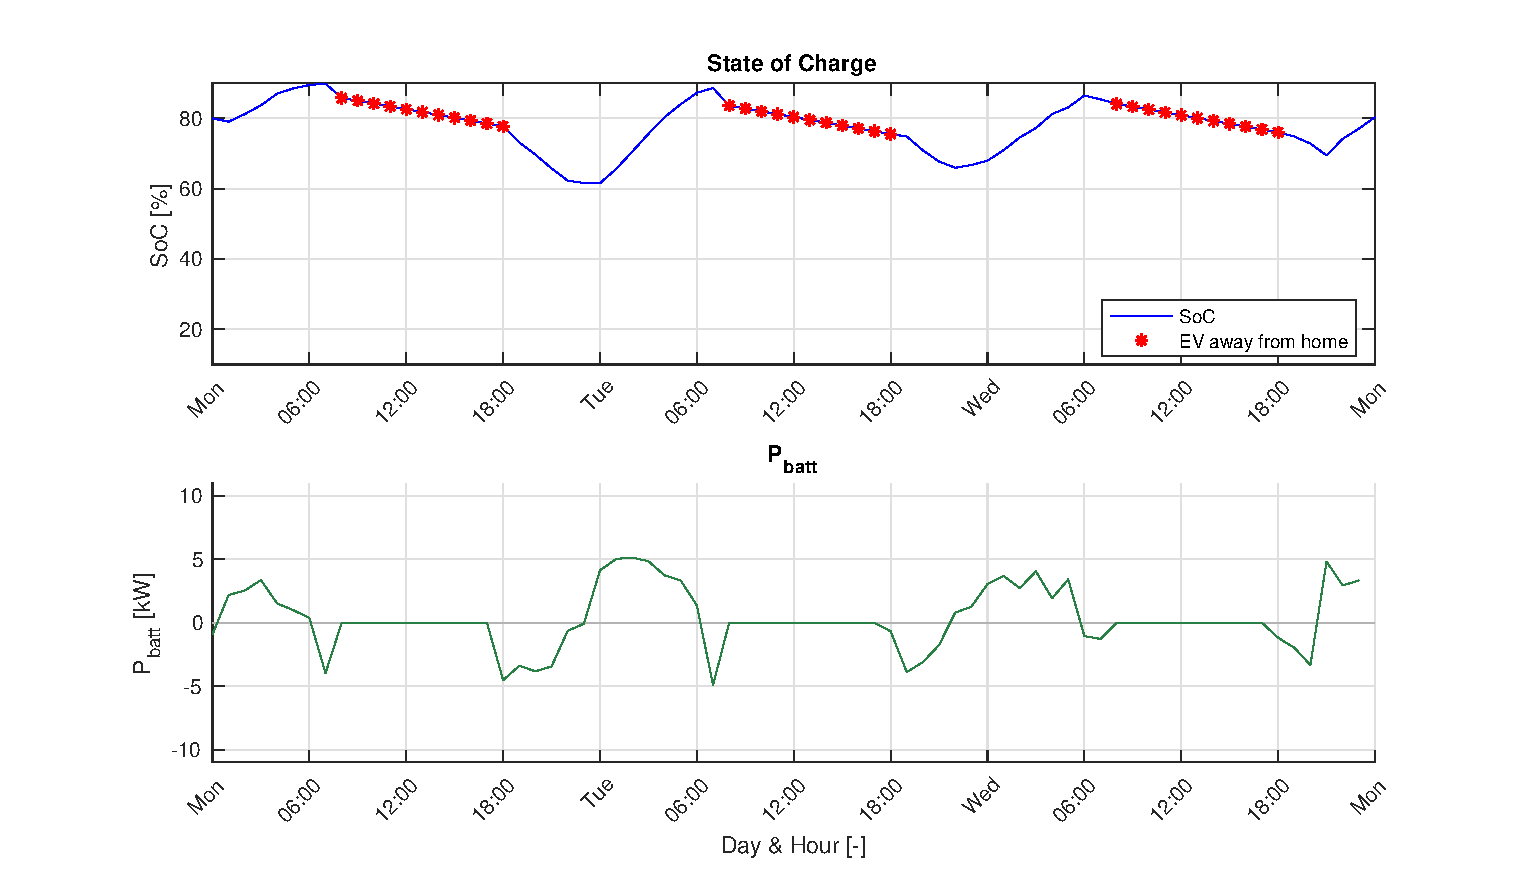
\includegraphics[scale = 0.5]{fig/soc6.eps} \\~\\
        Fall 2, med PV
    \end{figure}
    }
\end{frame}

% optiData6 voltage plot
\begin{frame}[plain]
\Wider[10em]{
    \begin{figure}
        \centering
        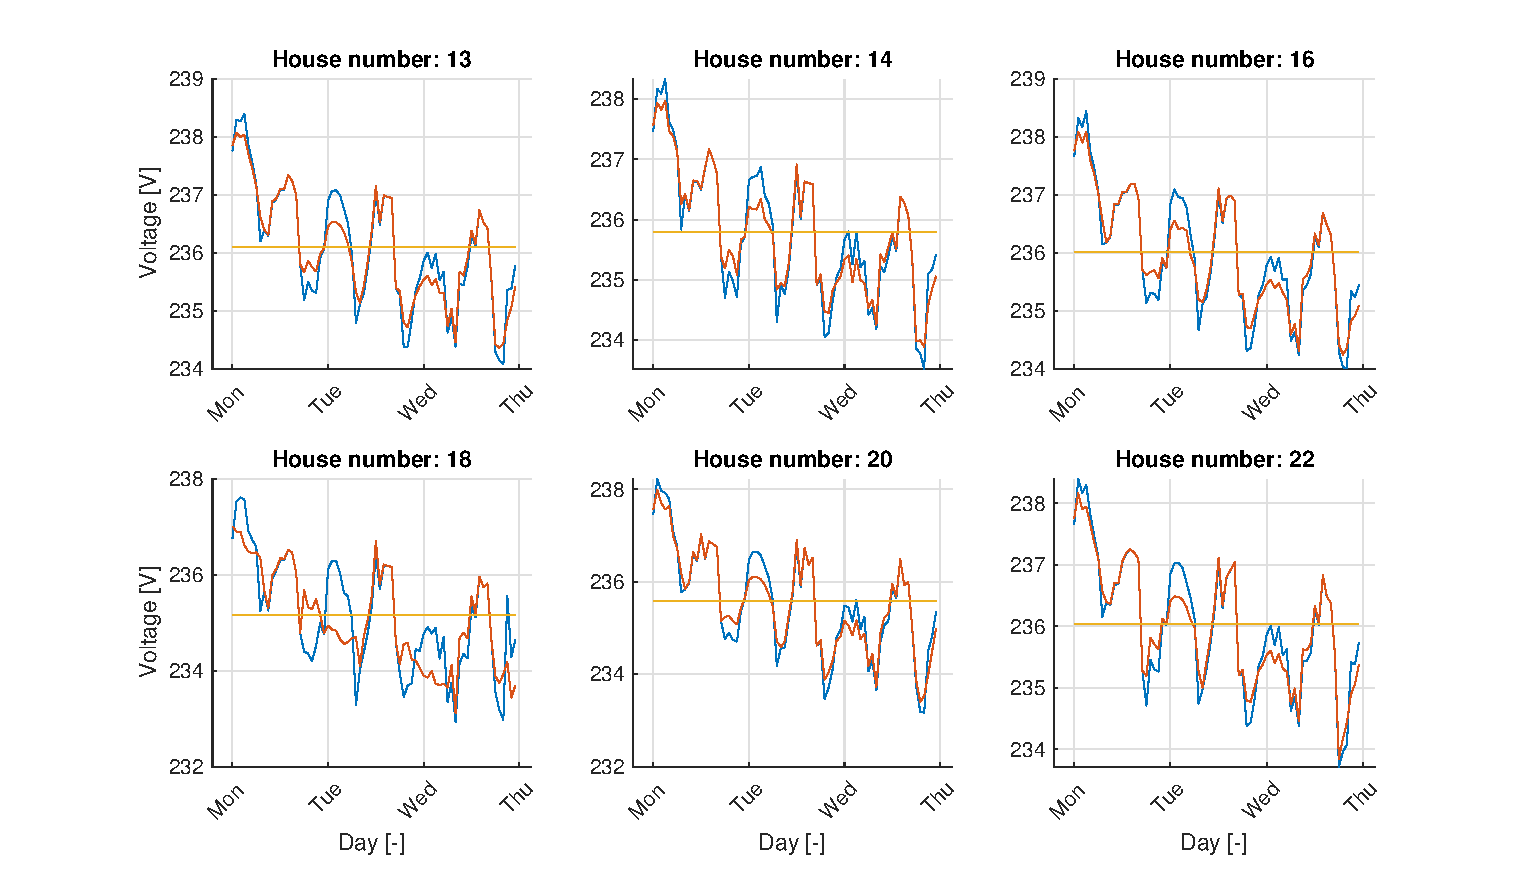
\includegraphics[scale = 0.5]{fig/volt6.eps} \\~\\
        Fall 2, med PV: \textcolor{myblue}{ej optimerad}, \textcolor{myred}{optimerad}, \textcolor{myyellow}{medelvärde}
    \end{figure}
    }
\end{frame}


%
\section{Kommande period}
\subsection{Utveckla fall 2}
\subsection{Fall 3}
\subsection{Justeringar och utökningar}
\subsection{Fall 4}
%

\begin{frame}
\frametitle{Utveckla fall 2}
    \begin{itemize}
        \item Addera fler elbilar. Både styrbara och icke-styrbara.
         
         \item Undersöka mer om placering av elbil i nätet.
         
         \item Justering av parametern $\beta$.
    \end{itemize}
\end{frame}

\begin{frame}
\frametitle{Fall 3}
    \begin{itemize}
        \item Inkludera icke-styrbara elbilar i nätet som laddas samtidigt.
        
        \item Antalet elbilar: samtliga hushåll har en eller procentsats baserad på prognoser från ex. Trafikanalys, Power Circle. 
        
        \item Maximal laddeffekt (trefas, 11kW). 
    \end{itemize}
\end{frame}

\begin{frame}
\frametitle{Justeringar och utökningar}
    \begin{enumerate}
         \item Andra körmönster för elbil. Idag använder vi medeldistans körd på en dag från 2017 (33km) från Trafikanalys och att bilen är otillgänglig mellan 08:00-17:00.
         
        \item Skapa ett specialanpassat, mindre elnät.
            \begin{itemize}
                \item[-] Använda data från Hallonvägen/Amundstorp
                \item[-] Unika lastprofiler för ex. skola, industri etc.
            \end{itemize}

        
      
        
        \item Skatta framtida konsumtion för hushållet utifrån historiska mätvärden. Kan vara av intresse för framtidens mätutrustning och eventuell implementering av algoritm. 
    \end{enumerate}
\end{frame}

\begin{frame}
\frametitle{Fall 4}
    \begin{itemize}
        \item Simulera ett stationärt batteri (går förvisso att göra i dagsläget). 
        
        \item Eventuell utökad batterimodell.
        
        \item Batteriplacering och antal batterier.
        
        \item Inkludera elbilar och solpaneler.
    \end{itemize}
\end{frame}

\section{Frågor och diskussion}


\end{document}